% !TEX program = xelatex
% ============================================================================
% មគ្គុទ្ទេសក៍ណែនាំការបង្រៀន និងរបាយការណ៍ស្រាវជ្រាវគរុកោសល្យ (Teaching Guideline -- EXP1)
% មុខវិជ្ជា៖ គណិតវិទ្យា ថ្នាក់ទី៨ -- ពីជគណិត មេរៀនទី២៖ ស្វ័យគុណ
% ចំណុចរង៖ ២.១ សញ្ញាណស្វ័យគុណ (ទំព័រ ១៣--១៤ និងលំហាត់ទំព័រ ២៥: #1, #3, #4)
% គ្រូបង្រៀន៖ ហុក ប៊ុនថែន | អនុវិទ្យាល័យព្រះក្រសាំង (កំពង់ស្វាយ-កំពង់ធំ)
% ============================================================================
\documentclass[a4paper,12pt]{article}

\usepackage[a4paper, left=1.45cm, right=1.45cm, top=2.30cm, bottom=2.30cm, headheight=18pt, headsep=0.68cm, footskip=0.88cm]{geometry}
\usepackage{amsmath, amssymb}
\usepackage{unicode-math}
\usepackage{fontspec}
\usepackage{array, longtable, multirow, colortbl, booktabs}
\usepackage[table]{xcolor}
\usepackage{enumitem}
\usepackage{pifont}
\usepackage{fancyhdr}
\usepackage{lastpage}
\usepackage{needspace}
\usepackage[hyphens]{url}
\usepackage{tikz}
\usepackage[most]{tcolorbox}
\usetikzlibrary{calc, arrows.meta, decorations.pathreplacing, positioning, babel}
\urlstyle{same}

\makeatletter
\let\@expl@@@mark@update@singlecol@structures@@\relax
\makeatother

% ============================================================================
% ការកំណត់ពុម្ពអក្សរ (Cross-Platform \NGSFindFonts: Windows Local + Cloud fonts/)
% ============================================================================
\providecommand{\NGSFindFonts}{%
  \IfFileExists{C:/Windows/Fonts/cambria.ttc}{%
    \def\NGSSysPath{C:/Windows/Fonts/}%
    \def\NGSUserPath{C:/Users/KIT/AppData/Local/Microsoft/Windows/Fonts/}%
  }{%
    \IfFileExists{./fonts/KhmerOSsiemreap.ttf}{\def\NGSSysPath{./fonts/}\def\NGSUserPath{./fonts/}}{%
    \IfFileExists{../fonts/KhmerOSsiemreap.ttf}{\def\NGSSysPath{../fonts/}\def\NGSUserPath{../fonts/}}{%
    \IfFileExists{../../fonts/KhmerOSsiemreap.ttf}{\def\NGSSysPath{../../fonts/}\def\NGSUserPath{../../fonts/}}{%
    \IfFileExists{../../../fonts/KhmerOSsiemreap.ttf}{\def\NGSSysPath{../../../fonts/}\def\NGSUserPath{../../../fonts/}}{%
    \IfFileExists{../../../../fonts/KhmerOSsiemreap.ttf}{\def\NGSSysPath{../../../../fonts/}\def\NGSUserPath{../../../../fonts/}}{%
    \IfFileExists{../../../../../fonts/KhmerOSsiemreap.ttf}{\def\NGSSysPath{../../../../../fonts/}\def\NGSUserPath{../../../../../fonts/}}{%
    \IfFileExists{../../../../../../fonts/KhmerOSsiemreap.ttf}{\def\NGSSysPath{../../../../../../fonts/}\def\NGSUserPath{../../../../../../fonts/}}{%
      \def\NGSSysPath{../../../../../../../fonts/}\def\NGSUserPath{../../../../../../../fonts/}%
    }}}}}}}%
  }%
}
\NGSFindFonts

\setmathfont[
  Path={\NGSSysPath},
  FontIndex=1,
  Scale=1.06
]{cambria.ttc}

\defaultfontfeatures{Ligatures=TeX}

\setmainfont[
  Path={\NGSUserPath},
  Extension=.ttf,
  Script=Khmer,
  BoldFont={KhmerOSsiemreap},
  BoldFeatures={FakeBold=1.8},
  ItalicFont={KhmerOSsiemreap},
  ItalicFeatures={FakeSlant=0.25},
  BoldItalicFont={KhmerOSsiemreap},
  BoldItalicFeatures={FakeBold=1.8, FakeSlant=0.25}
]{KhmerOSsiemreap}

% ហាមដាក់ FakeBold លើ KhmerOSmuollight និងហាមរុំ \muol ក្នុង \textbf{...}
\newfontfamily\muol[
  Path={\NGSUserPath},
  Extension=.ttf,
  Script=Khmer
]{KhmerOSmuollight}

\newfontfamily\TimesEn[
  Path={\NGSSysPath},
  Extension=.ttf,
  Scale=1.02,
  BoldFont={timesbd},
  ItalicFont={timesi},
  BoldItalicFont={timesbi}
]{times}

\newfontfamily\Tacteing[
  Path={\NGSUserPath}
]{TACTENG.TTF}

\newfontfamily\CourierBullet[
  Path={\NGSSysPath},
  Extension=.ttf
]{cour}

% ក្បួនកាត់ពាក្យខ្មែរ (Khmer word wrapping)
\XeTeXlinebreaklocale "km"
\XeTeXlinebreakskip = 0pt plus 1pt minus 0.1pt

% Mobile-First comfortable line spacing (11.5pt / 18.2pt effective)
\linespread{1.22}

% ============================================================================
% ពណ៌ ស-ខ្មៅ (Strict Monochrome Grayscale Palette) & Fancyhdr
% ============================================================================
\definecolor{headgray}{HTML}{F2F2F2}
\definecolor{panelgray}{gray}{0.94}
\definecolor{stepgray}{HTML}{D9D9D9}
\definecolor{midgray}{gray}{0.82}
\definecolor{bordergray}{gray}{0.45}

\pagestyle{fancy}
\fancyhf{}
\renewcommand{\headrulewidth}{0.4pt}
\renewcommand{\footrulewidth}{0.4pt}
\fancyhead[L]{\rule[-3pt]{0pt}{14pt}\fontsize{9.5pt}{13pt}\selectfont មគ្គុទ្ទេសក៍ណែនាំការបង្រៀន \en{(Grade 8 EXP1)}}
\fancyhead[R]{\rule[-3pt]{0pt}{14pt}\fontsize{9.5pt}{13pt}\selectfont មេរៀនទី២ \en{(}២\en{.}១\en{)}៖ សញ្ញាណស្វ័យគុណ}
\fancyfoot[L]{\rule{0pt}{13pt}\fontsize{9.5pt}{13.5pt}\selectfont កញ្ចប់ឯកសារ \en{NGS 5Es} \en{(}៥០ នាទី\en{)} \en{|} ហុក ប៊ុនថែន}
\fancyfoot[R]{\rule{0pt}{13pt}\fontsize{9.5pt}{13.5pt}\selectfont ទំព័រ \en{\thepage\ / \pageref{LastPage}}}

\fancypagestyle{firstpage}{%
  \fancyhf{}%
  \renewcommand{\headrulewidth}{0pt}%
  \renewcommand{\footrulewidth}{0.4pt}%
  \fancyfoot[L]{\rule{0pt}{13pt}\fontsize{9.5pt}{13.5pt}\selectfont កញ្ចប់ឯកសារ \en{NGS 5Es} \en{(}៥០ នាទី\en{)} \en{|} អនុវិទ្យាល័យព្រះក្រសាំង}%
  \fancyfoot[R]{\rule{0pt}{13pt}\fontsize{9.5pt}{13.5pt}\selectfont ទំព័រ \en{\thepage\ / \pageref{LastPage}}}%
}

\setlength{\parindent}{0pt}
\setlength{\parskip}{3.0pt}
\setlength{\tabcolsep}{4pt}
\setlength{\emergencystretch}{2em}
\setlist{itemsep=2.2pt, parsep=0pt}

% ============================================================================
% ម៉ាក្រូជំនួយ និងឋានានុក្រម \muol គ្មានតួអក្សរ ASCII បន្លំ (0 Missing character)
% ============================================================================
\newcommand{\en}[1]{{\TimesEn #1}}
\newcommand{\enbf}[1]{{\TimesEn\textbf{#1}}}
\newcommand{\enit}[1]{{\TimesEn\textit{#1}}}
\newcommand{\unit}[1]{\,\text{\en{#1}}}
\newcommand{\cnum}[1]{{\TimesEn\fontsize{10.5pt}{12pt}\selectfont\ding{\numexpr181+#1\relax}}}
\newcommand{\ditem}{\tikz[baseline=-0.5ex]\fill (0,0.40ex) -- (0.40ex,0) -- (0,-0.40ex) -- (-0.40ex,0) -- cycle;\hspace{0.25em}}
\newcommand{\wcirc}{{\CourierBullet\fontsize{9.8pt}{11pt}\selectfont o}}
\newcommand{\chkbox}{\tikz[baseline=-0.15ex]\draw[black, line width=0.85pt] (0,0) rectangle (0.25cm,0.25cm);}
\newcommand{\lockbox}[1]{\tikz[baseline=(X.base)]\node[draw=black, line width=0.85pt, fill=panelgray, inner sep=1.8pt, anchor=base] (X) {$#1$};}
\newcommand{\khmflourish}{{\Tacteing\fontsize{38pt}{15pt}\selectfont\raisebox{-5pt}{3}}}

\newcommand{\parttitle}[1]{{\muol\fontsize{13.5pt}{18pt}\selectfont #1}}
\newcommand{\sectitle}[1]{{\muol\fontsize{12pt}{16pt}\selectfont #1}}
\newcommand{\subsectitle}[1]{{\muol\fontsize{11.5pt}{15.5pt}\selectfont #1}}
\newcommand{\tblhead}[1]{{\muol\fontsize{10.2pt}{15.6pt}\selectfont #1\par}}

\newcolumntype{L}[1]{>{\raggedright\arraybackslash}p{#1}}
\newcolumntype{C}[1]{>{\centering\arraybackslash}p{#1}}
\newcolumntype{R}[1]{>{\raggedleft\arraybackslash}p{#1}}

\newcommand{\secbanner}[2]{%
  \Needspace{2.1cm}%
  \vspace{1pt}%
  \begin{tcolorbox}[
    enhanced, sharp corners, colback=stepgray, colframe=black,
    boxrule=1.05pt, borderline south={0.6pt}{1.8pt}{black},
    top=4pt, bottom=4pt, left=9pt, right=9pt,
    before skip=3pt, after skip=3pt
  ]
    \sectitle{#1}\\[2pt]
    {\fontsize{10pt}{12.5pt}\selectfont\enit{#2}}%
  \end{tcolorbox}%
}

\newcommand{\refbanner}[1]{%
  \Needspace{2.1cm}%
  \vspace{2pt}%
  \begin{tcolorbox}[
    enhanced, sharp corners, colback=headgray, colframe=black,
    boxrule=0.85pt, borderline south={0.6pt}{1.8pt}{black},
    top=6pt, bottom=6pt, left=9pt, right=9pt,
    before skip=3pt, after skip=4pt
  ]
    {\muol\fontsize{12pt}{19pt}\selectfont #1}%
  \end{tcolorbox}%
}

\newcommand{\subsec}[1]{%
  \Needspace{1.6cm}%
  \vspace{2pt}%
  \subsectitle{#1}\par%
  \vspace{-2pt}%
  {\color{black}\hrule height 0.55pt}%
  \vspace{2pt}%
}

\newtcolorbox{phasebox}[3]{%
  enhanced, breakable, sharp corners,
  colback=white, colframe=black,
  boxrule=1.0pt, top=4pt, bottom=4pt, left=9pt, right=9pt,
  toptitle=3pt, bottomtitle=3pt,
  before skip=4pt, after skip=0pt,
  colbacktitle=headgray, coltitle=black,
  fonttitle=\fontsize{11pt}{14.5pt}\selectfont,
  fontupper=\fontsize{11.5pt}{15.0pt}\selectfont,
  title={%
    \linespread{1.0}\selectfont\renewcommand{\arraystretch}{1.0}%
    \begin{tabular*}{\linewidth}{@{}>{\raggedright\arraybackslash}p{13.55cm}@{\extracolsep{\fill}}r@{}}
      {\muol\fontsize{11pt}{14.5pt}\selectfont #1} & {\fontsize{10.5pt}{13.5pt}\selectfont\en{#2 |} #3}%
    \end{tabular*}%
  }
}

\newtcolorbox{scriptbox}{%
  enhanced, breakable, sharp corners, colback=panelgray, colframe=black,
  boxrule=0.8pt, borderline west={2.4pt}{0pt}{black},
  top=4.5pt, bottom=4.5pt, left=9pt, right=8pt,
  before skip=-0.8pt, after skip=4pt,
  fontupper=\fontsize{11.5pt}{15.0pt}\selectfont
}

\begin{document}
\thispagestyle{firstpage}
\fontsize{11.5pt}{15.0pt}\selectfont
\vspace*{-0.75cm}

% ============================================================================
% ក្បាលលិខិតផ្លូវការថ្នាក់ជាតិ & សាលារៀន (Kampong Thom / Kampong Svay / Preah Krasang)
% ============================================================================
{\linespread{1.08}\selectfont
\begin{center}
  {\muol\fontsize{12pt}{15.5pt}\selectfont ព្រះរាជាណាចក្រកម្ពុជា}\\[2pt]
  {\muol\fontsize{12pt}{15.5pt}\selectfont ជាតិ សាសនា ព្រះមហាក្សត្រ}\\[1pt]
  \khmflourish
\end{center}
\vspace{-4pt}
{\muol\fontsize{10.8pt}{15.5pt}\selectfont
  មន្ទីរអប់រំ យុវជន និងកីឡា ខេត្តកំពង់ធំ\\
  ការិយាល័យអប់រំ យុវជន និងកីឡា ស្រុកកំពង់ស្វាយ\\
  អនុវិទ្យាល័យព្រះក្រសាំង\par}
\vspace{4pt}
\begin{center}
  \parttitle{មគ្គុទ្ទេសក៍ណែនាំការបង្រៀន និងផែនការគរុកោសល្យ \enbf{(Teaching Guide)}}\\[3pt]
  {\fontsize{11.0pt}{14.5pt}\selectfont\textbf{ពីជគណិត មេរៀនទី២៖ ស្វ័យគុណ \en{---} ២\en{.}១ សញ្ញាណស្វ័យគុណ \en{(}ទំព័រ ១៣\en{--}១៤ និង ២៥\en{)}}}
\end{center}
}

\vspace{2pt}
\begin{tcolorbox}[
  enhanced, sharp corners, colback=headgray, colframe=black,
  boxrule=0.85pt, top=5pt, bottom=5pt, left=7pt, right=7pt,
  before skip=2pt, after skip=4pt
]
  \linespread{1.08}\fontsize{10.5pt}{14pt}\selectfont
  \renewcommand{\arraystretch}{1.15}
  \begin{tabular}{@{}L{3.10cm}@{}C{0.25cm}@{}L{5.10cm}@{\hspace{0.25cm}}L{2.65cm}@{}C{0.25cm}@{}L{5.75cm}@{}}
    \textbf{\en{-} មុខវិជ្ជា \en{/} ថ្នាក់} & \en{:} & គណិតវិទ្យា \en{(}ថ្នាក់ទី៨\en{)} & \textbf{\en{-} កាលបរិច្ឆេទ} & \en{:} & ថ្ងៃចន្ទ ទី១៦ ខែវិច្ឆិកា ឆ្នាំ២០២៦ \\
    \textbf{\en{-} ផ្នែក \en{/} មេរៀន} & \en{:} & ពីជគណិត \en{/} មេរៀនទី២៖ ស្វ័យគុណ & \textbf{\en{-} រយៈពេល} & \en{:} & ៥០ នាទី \en{(}១ ម៉ោងសិក្សា\en{)} \\
    \textbf{\en{-} ចំណុចរង} & \en{:} & ២\en{.}១ សញ្ញាណស្វ័យគុណ & \textbf{\en{-} សៀវភៅគោល} & \en{:} & ទំ\en{.} ១៣\en{--}១៤\en{,} ២៥ \en{(\#1, \#3, \#4)} \\
    \textbf{\en{-} បង្រៀនដោយ} & \en{:} & ហុក ប៊ុនថែន & \textbf{\en{-} ភស្តុតាងយោង} & \en{:} & ១៥ អត្ថបទ \en{Open-Access PDFs}
  \end{tabular}
\end{tcolorbox}

% ============================================================================
% ផ្នែកទី ១៖ បរិបទមេរៀន ការវិភាគសៀវភៅគោល និងផែនការលម្អិត ៥០ នាទី
% ============================================================================
\secbanner{ផ្នែកទី ១៖ បរិបទមេរៀន និងផែនការបង្រៀនលម្អិត ៥០ នាទី}{Section 1: Preah Krasang Classroom Context, Textbook Scope Audit \& Detailed 50-Minute Instructional Plan}

\subsec{១\enbf{.}១ បរិបទអនុវិទ្យាល័យព្រះក្រសាំង វិសាលភាពមេរៀន និងបញ្ហាប្រឈមស្នូលទាំង ៣}

ចំណុចរង \textbf{២\en{.}១ «សញ្ញាណស្វ័យគុណ»} (សៀវភៅសិក្សាគោលថ្នាក់ទី៨ ទំព័រ ១៣\en{--}១៤ និងលំហាត់ចុងមេរៀនទំព័រ ២៥) ជាម៉ោងសិក្សាបើកឆាកដ៏សំខាន់បំផុតនៃមេរៀនទី២ បន្ទាប់ពីសិស្សទើបបញ្ចប់ \textbf{មេរៀនទី១៖ ចំនួនសនិទាន} (ការគុណចំនួនសនិទានមានសញ្ញា និងប្រភាគ ទំព័រ ១១\en{--}១២) ហើយជាគ្រឹះផ្ទាល់សម្រាប់ចំណុច \textbf{២\en{.}២ វិធីគុណ និងចែកស្វ័យគុណគោលដូចគ្នា} (ទំព័រ ១៥\en{--}១៩)។ ការពិនិត្យផ្ទៀងផ្ទាត់សៀវភៅគោលទំព័រ ១៣\en{--}១៤ និង ២៥ រួមជាមួយភស្តុតាងស្រាវជ្រាវអន្តរជាតិ \en{Open-Access} ចំនួន ១៥ ច្បាប់ បង្ហាញបញ្ហាប្រឈមស្នូល ៣ ប្រការដែលគ្រូត្រូវដោះស្រាយក្នុងរយៈពេល ៥០ នាទី៖
\begin{itemize}[leftmargin=0.65cm]
  \item \textbf{១\en{.} អន្ទាក់គុណលីនេអ៊ែរ ($a^n = a\times n$) អន្ទាក់បូកតួដូចគ្នា ($a+a=a^2$) និងការប្ដូរគោល-និទស្សន្ត៖} ការសិក្សាលើសិស្សថ្នាក់ទី៨ ចំនួន \en{N = 165} នាក់បង្ហាញថា មានតែ \en{3.5\%} ប៉ុណ្ណោះធ្វើលំហាត់ស្វ័យគុណត្រូវគ្រប់ខ្ទង់ ខណៈសិស្សជាច្រើនយកគោលគុណនិទស្សន្ត ($2^4=8, 2^6=12$) ឬប្ដូរតួនាទីគោលនឹងនិទស្សន្ត ($2^6=6\times 6=36$) \en{(Ulusoy, 2019)}។ ស្របគ្នានេះ សិស្សថ្នាក់ទី៨ ដល់ទៅ \en{63.2\%} ច្រឡំសរសេរ $d+d=d^2$ ដោយលាយឡំផលបូកតួដូចគ្នា ($2d$) ជាមួយផលគុណកត្តាដូចគ្នា ($d\cdot d$) \en{(Moru \& Mathunya, 2022)} ហើយមានតែ \en{23\%} ប៉ុណ្ណោះដែលឆ្លងផុតអារម្មណ៍បំភាន់លីនេអ៊ែរ \en{(De Bock et al., 2003)}។
  \item \textbf{២\en{.} កំហុសសញ្ញាដកលើវង់ក្រចក \en{$(-a)^n$ vs $-a^n$} គោលប្រភាគ \en{$(a/b)^n$} និងលំដាប់ប្រមាណវិធី៖} កំហុសសញ្ញាដកគឺជាកំហុសលេខ ១ ដែលកើតឡើងញឹកញាប់ជាងគេបំផុតក្នុងពីជគណិតថ្នាក់ទី៨ \en{(Booth et al., 2014, p < .001)}។ សិស្ស \en{30.9\%} មើលរំលងវង់ក្រចកដោយសន្មតខុសថា «ឱ្យតែនិទស្សន្តគូ លទ្ធផលវិជ្ជមានជានិច្ច» រហូតសរសេរ $-2^4 = (-2)^4 = +16$ \en{(Ulusoy, 2019; Theba et al., 2024)} ខណៈហានិភ័យខុសអាទិភាពប្រមាណវិធីកើនឡើង \en{3.28} ដងពេលសញ្ញាដកនៅខាងឆ្វេងបំផុត \en{(Bye et al., 2024; Tabak, 2019)} និងងាយភ្លេចលើកភាគបែងក្នុងប្រភាគ $(\frac{2}{3})^3 \to \frac{8}{3}$ \en{(Lee \& Boyadzhiev, 2020)}។
  \item \textbf{៣\en{.} កំហុសបោះពុម្ព និងគម្លាតលំហាត់ទាំង ៤ ចំណុចក្នុងសៀវភៅគោល (ទំ\en{.}១៣\en{--}១៤ និង ២៥)៖} \textbf{(i) ទំ\en{.}១៣} បន្ទាត់ទី ១៤ បោះពុម្ពខុសថា \en{$8^2$} ផ្ទុយពីចំណុចរងទី ៣ ដែលអានថា \en{$8^4$}; \textbf{(ii) ទំ\en{.}១៤} ប្រអប់និយមន័យកំណត់ $n$ ជា «ចំនួនគត់រ៉ឺឡាទីបខុសពីសូន្យ» ($\mathbb{Z}^*$) ដែលរួមបញ្ចូលទាំងចំនួនគត់អវិជ្ជមាន ($-1, -2, \dots$) ធ្វើឱ្យឃ្លា «$n$ កត្តា» គ្មានន័យគណិតវិទ្យា \en{(Sureda \& Otero, 2019)} (ត្រូវបញ្ជាក់ $n$ ជាចំនួនគត់វិជ្ជមាន $n\ge 1$ សម្រាប់និយមន័យ $n$ កត្តា); \textbf{(iii) ទំ\en{.}១៤} លំហាត់គំរូទី ២ បាត់សញ្ញា «។» គ្នាបក្រោម \en{$(-2)^6$} ដាច់ជា ២ កំណាត់ សម្គាល់ \en{$(-1)^n$} មិនព្រមានរឿងវង់ក្រចក ហើយប្រតិបត្តិ ១ ប្ដូរសញ្ញាគុណពី $\times$ មកចំណុចកណ្ដាល $\cdot$ ដោយគ្មានការពន្យល់; និង \textbf{(iv) ទំ\en{.}២៥} លំហាត់ \en{\#2} និង \en{\#3} បញ្ចេញទម្រង់ថ្មី \en{$(-3^2), (-5^2), (-8^2)$} (និទស្សន្តនៅក្នុងវង់ក្រចកលើតែលេខវិជ្ជមាន ស្មើនឹង $-9, -25, -64$) ដែលមិនធ្លាប់បង្ហាញសោះលើទំព័រ ១៣\en{--}១៤!
\end{itemize}

ដើម្បីដោះស្រាយបញ្ហាទាំង ៣ នេះ មគ្គុទ្ទេសក៍នេះរៀបចំផែនការបង្រៀន ៥០ នាទី \en{(2 + 9 + 17 + 20 + $\le$2 min)} តាមគោលការណ៍ភាពថ្មីជានិច្ច ដោយឱ្យសិស្សដើរតួជា \textbf{«ក្រុមអ្នកស៊ើបអង្កេតកូដស្វ័យគុណ និងបន្ទះបត់ទ្វេដង»} ប្រើពិសោធន៍បត់ក្រដាសផ្ទាល់ដៃ ($2^1\to 2^6=64$ ស្រទាប់), \textbf{ប្រអប់ចាក់សោវង់ក្រចក ស-ខ្មៅ} \lockbox{-2}, ការអូសម្រាមដៃ \en{\textbf{[tracing]}} ផ្គូផ្គងគូសញ្ញាដក \en{(Yeo \& Tzeng, 2019)}, លំហាត់គំរូប្រៀបធៀបត្រូវ-ខុស \en{(Booth et al., 2013)}, និង\textbf{ធនាគារហេតុផល \cnum{1}\en{--}\cnum{5}} តាមរចនាសម្ព័ន្ធ \en{Hub-and-Spoke (Xu et al., 2026)}។

\subsec{១\enbf{.}២ ផែនការលម្អិតសម្រាប់ម៉ោងសិក្សា ៥០ នាទី \enbf{(2 + 9 + 17 + 20 + $\le$2 min)} តាមគំរូ \enbf{5Es}}

តារាងខាងក្រោមបង្ហាញផែនការមេលម្អិតនៃម៉ោងសិក្សា ១ ម៉ោង (៥០ នាទី) សម្រាប់ចំណុច ២\en{.}១ ព្រមទាំងការតភ្ជាប់ទៅកាន់គម្រោងសម្ភារៈបោះពុម្ព ស-ខ្មៅ (ទំព័រ ១\en{--}៦) ដែលនឹងប្រើនៅពេលរៀបចំកិច្ចតែងការបង្រៀនក្នុងជំហានបន្ទាប់៖

\begingroup
\linespread{1.04}\fontsize{10.2pt}{14.5pt}\selectfont
\renewcommand{\arraystretch}{1.08}
\begin{longtable}{|C{2.45cm}|L{3.55cm}|L{8.35cm}|C{2.50cm}|}
\hline
\rowcolor{headgray}
\multicolumn{1}{|C{2.45cm}|}{\tblhead{ជំហាន \enbf{/} ពេល}} &
\multicolumn{1}{C{3.55cm}|}{\tblhead{ដំណាក់កាល \enbf{\&} សកម្មភាព}} &
\multicolumn{1}{C{8.35cm}|}{\tblhead{ខ្លឹមសារស្នូល សកម្មភាពគ្រូ\enbf{-}សិស្ស និងគោលដៅគរុកោសល្យ}} &
\multicolumn{1}{C{2.50cm}|}{\tblhead{សម្ភារៈគាំទ្រ}} \\
\hline
\endfirsthead
\hline
\rowcolor{headgray}
\multicolumn{1}{|C{2.45cm}|}{\tblhead{ជំហាន \enbf{/} ពេល}} &
\multicolumn{1}{C{3.55cm}|}{\tblhead{ដំណាក់កាល \enbf{\&} សកម្មភាព}} &
\multicolumn{1}{C{8.35cm}|}{\tblhead{ខ្លឹមសារស្នូល សកម្មភាពគ្រូ\enbf{-}សិស្ស និងគោលដៅគរុកោសល្យ}} &
\multicolumn{1}{C{2.50cm}|}{\tblhead{សម្ភារៈគាំទ្រ}} \\
\hline
\endhead
\hline
\endfoot
\hline
\endlastfoot
\textbf{ជំហានទី ១} \newline \en{00--02 min (2')} & រដ្ឋបាលថ្នាក់ & ពិនិត្យវត្តមាន សណ្ដាប់ធ្នាប់ ចាត់ក្រុម ៣ នាក់ជា «ក្រុមអ្នកស៊ើបអង្កេតកូដស្វ័យគុណ» ចែកបន្ទះក្រដាសបត់ និងសន្លឹកពិសោធន៍ទំព័រ ១ ផ្កាប់លើតុ។ & បន្ទះក្រដាស \en{\&} ទំព័រ ១ \en{(}ផ្កាប់\en{)} \\
\hline
\textbf{ជំហានទី ២ក} \newline \en{02--05 min (3')} & កែកិច្ចការផ្ទះចាស់ & កែខ្លីមេរៀនទី១ ចំនួនសនិទាន ទំ\en{.}១២ \en{\#10}ក\en{, \#10}ច និងទំ\en{.}១១ \en{\#4}គ៖ រំលឹកក្បួនសញ្ញា $(-)\times(-)=(+)$, $(-)\times(-)\times(-)=(-)$ និងគុណប្រភាគ $\frac{a}{b}\times\frac{c}{d}=\frac{ac}{bd}$។ & ក្តារខៀនឆ្វេង \\
\hline
\textbf{ជំហានទី ២ខ} \newline \en{05--08 min (3')} & រំលឹកមេរៀនទាក់ទង & ប្រៀបធៀប \textbf{ផលបូកតួដូចគ្នា} ($4+4+4=4\times 3=12$; $d+d=2d$) ទល់នឹង \textbf{ផលគុណកត្តាដូចគ្នា} តាមឧទាហរណ៍ទំ\en{.}១៣ អាកាសយានដ្ឋាន $10\,000 = 10\times 10\times 10\times 10$។ & ក្តារខៀនឆ្វេង \en{\&} ទំ\en{.}១៣ \\
\hline
\textbf{ជំហានទី ២គ} \newline \textbf{\en{E1 Engage}} \newline \en{08--11 min (3')} & បេសកកម្មបត់ក្រដាស ៦ ដង \en{\&} កូដសញ្ញាដក & ចោទបញ្ហាភ្ញាក់ផ្អើល ២៖ \textbf{(១)} បត់ក្រដាសជា ២ ស្មើៗគ្នា \textbf{៦ ដងជាប់គ្នា} តើបាន $12$ ស្រទាប់ ($2\times 6$) ឬ $64$ ស្រទាប់? \textbf{(២)} តើ $(-2)^6$ និង $-2^6$ ឱ្យតម្លៃស្មើគ្នា ឬផ្ទុយសញ្ញាគ្នា? (ស្ទង់មតិកត់លើក្ដារខៀន មិនទាន់លាតចម្លើយ)។ & បន្ទះក្រដាសគ្រូ \en{\&} ក្តារខៀន \\
\hline
\textbf{ជំហានទី ៣ក} \newline \textbf{\en{E2 Explore}} \newline \en{11--22 min (11')} & \en{POE 1} បត់ក្រដាស \en{(6')} \en{\& POE 2} ប្រអប់ចាក់សោ \en{(5')} & \textbf{សកម្មភាព ១ (\en{6'})}៖ ទស្សន៍ទាយ (\en{P}), បត់ក្រដាសផ្ទាល់ដៃកត់ត្រាស្រទាប់ $1\to 2, 2\to 4, 3\to 8, 4\to 16, 5\to 32, 6\to 64\neq 12$ (\en{O}), ពន្យល់ (\en{E}) កម្ទេចអន្ទាក់ $a^n=a\times n$ និង $a+a=a^2$។ \newline \textbf{សកម្មភាព ២ (\en{5'})}៖ អូស \en{[tracing]} លើប្រអប់ចាក់សោ $\lockbox{-2}^6 = +64$ (ផ្គូផ្គងដក ៣ គូ) ទល់នឹង $-2^6 = -(2^6) = -64$, $(-3)^3 = -27$ និង $(\frac{2}{3})^3 = \frac{8}{27} \neq \frac{2^3}{3} = \frac{8}{3}$។ & ទំព័រ ១ \en{(1:1)} \en{\&} បន្ទះបត់ \\
\hline
\textbf{ជំហានទី ៣ខ} \newline \textbf{\en{E3 Explain}} \newline \en{22--28 min (6')} & បង្គុំនិយមន័យ កែទំ\en{.}១៣\en{--}១៤ \en{\&} ផ្ទាំង \cnum{1}\en{--}\cnum{5} & សំយោគ \textbf{គោល ($a$)}, \textbf{និទស្សន្ត ($n$)}, \textbf{ស្វ័យគុណ ($a^n$)}, ការអានការេ-គូប (\textbf{កែទំ\en{.}១៣ \en{Erratum \#1}: $8^2\to 8^4$}), និយមន័យ $\underbrace{a\times\dots\times a}_{n\text{ កត្តា}}=a^n$ (\textbf{កែទំ\en{.}១៤ \en{Erratum \#2}: $n$ គត់វិជ្ជមាន $n\ge 1$, $a^1=a$}), សម្គាល់ $(-1)^n$ និងបិទផ្ទាំង \textbf{ធនាគារហេតុផល \cnum{1}\en{--}\cnum{5}}។ & សៀវភៅទំ\en{.}១៣\en{--}១៤ \en{\&} ទំព័រ ៤ \\
\hline
\textbf{ជំហានទី ៤ក} \newline \textbf{\en{E4 Elaborate}} \newline \en{28--38 min (10')} & កាតស៊ើបអង្កេត លំហាត់គំរូទី ១\en{--}២ \en{\& EIA 30s} & អនុវត្តកាត ៣ ជំហាន + \en{[tracing]} លើ \textbf{លំហាត់គំរូទី ១} ($4^6, a^{2010}$) និង \textbf{លំហាត់គំរូទី ២} ($2^5=32$, $(\frac{2}{3})^3=\frac{8}{27}$, $(-3)^3=-27$, $(-2)^6=64$ \textbf{កែ \en{Erratum \#3}} ធៀបផ្ទាល់នឹង $-2^6=-64$ និង $(-3^2)=-9$) + សំណួរឆ្លុះបញ្ចាំង \en{EIA 30s}។ & ទំព័រ ២ \en{(2-up)} \\
\hline
\textbf{ជំហានទី ៤ខ} \newline \textbf{\en{E5 Evaluate}} \newline \en{38--48 min (10')} & \en{Relay} ប្រតិបត្តិ ១\en{--}២ \en{(6.5')} \en{\&} កាត \en{A--D (3.5')} & \textbf{\en{Relay} ៣ តួនាទី (\en{6.5'})}៖ ប្រតិបត្តិ ១ ($x^6, y^{2013}$ ពន្យល់សញ្ញា $\cdot$) និងប្រតិបត្តិ ២ ($3^4=81, (-\frac{1}{2})^6=\frac{1}{64}, (-2)^7=-128$) + \en{Pause-Ask / Pause-Review!} + \textbf{ឆ្លើយបិទ \en{E1}}។ \textbf{វាយតម្លៃរហ័ស (\en{3.5'})}៖ កាត \en{A--D} + សំបុត្រចេញ ៣ សំណួរ (៦០\en{--}៩០ វិនាទី)។ & ទំព័រ ៣ \en{\&} ទំព័រ ៥ \\
\hline
\textbf{ជំហានទី ៥} \newline \en{48--50 min ($\le$2')} & កិច្ចការផ្ទះទំ\en{.}២៥ \en{\&} បណ្ដាំមេរៀនបន្ត & ដាក់កិច្ចការផ្ទះទំ\en{.}២៥៖ \textbf{\en{\#1}(ក\en{--}ឃ)}, \textbf{\en{\#3}(ក\en{,} ខ\en{,} ឃ)} (\textbf{ព្រមាន \en{Alert \#4}: $(-3^2)=-(3^2)=-9$!}) និង \textbf{\en{\#4}} ($b=3 \Rightarrow P=72$); ផ្ដាំអានមុនចំណុច \textbf{២\en{.}២} (ទំ\en{.}១៥\en{--}១៦)។ & ទំព័រ ៦ \en{(4-up)} \\
\hline
\end{longtable}
\endgroup

% ============================================================================
% ផ្នែកទី ២៖ ការសំយោគឯកសារស្រាវជ្រាវអន្តរជាតិ (Mini-Literature Review)
% ============================================================================
\secbanner{ផ្នែកទី ២៖ ការសំយោគឯកសារស្រាវជ្រាវអន្តរជាតិ \enbf{(Mini-Literature Review)}}{Section 2: Empirical Synthesis Across 15 Verified Open-Access Algebra \& Cognitive Studies}

\subsec{២\enbf{.}១ ឧបសគ្គការយល់ដឹងលើស្វ័យគុណ៖ អន្ទាក់គុណ\enbf{-}បូក ការប្ដូរគោល និងដែននិយមន័យ \enbf{(E1--E3)}}

ការបង្រៀនសញ្ញាណស្វ័យគុណដោយចាប់ផ្ដើមត្រឹមការឱ្យសិស្សទន្ទេញនិយមន័យ $a^n$ តាមបែបប្រពៃណី មិនអាចទប់ស្កាត់កំហុសគោលគំនិតដ៏រ៉ាំរ៉ៃរបស់សិស្សមធ្យមសិក្សាបឋមភូមិបានឡើយ។ \en{Ulusoy (2019, pp. 56--59)} បានធ្វើតេស្តលើសិស្សថ្នាក់ទី៨ ចំនួន \en{N = 165} នាក់លើកន្សោមស្វ័យគុណ ១០ ខ្ទង់ និងសម្ភាសន៍គ្លីនិកចំនួន \en{12} នាក់ ហើយរកឃើញថា មានសិស្សត្រឹមតែ \en{3.5\%} ប៉ុណ្ណោះដែលឆ្លើយត្រូវគ្រប់ខ្ទង់ទាំងអស់! ទោះបីសិស្ស \en{73.3\%} គណនា $2^4=16$ បានត្រូវ ក៏មានសិស្ស \en{4\% (n = 7)} គណនាតាមអន្ទាក់គុណលីនេអ៊ែរ $a^n = a\cdot n$ ($2^4 = 2\cdot 4 = 8$ និង $2^6 = 2\cdot 6 = 12$) រីឯសិស្ស \en{6.7\% (n = 11)} ប្ដូរតួនាទីគោលនឹងនិទស្សន្ត ($2^6 = 6\cdot 6 = 36$ និង $3^5 = 5\cdot 5\cdot 5 = 125$)។ កាន់តែធ្ងន់ធ្ងរជាងនេះ \en{Moru \& Mathunya (2022, Table 2, p. 137)} បានវិភាគសន្លឹកកិច្ចការពីជគណិតសិស្សថ្នាក់ទី៨ ចំនួន \en{N = 95} នាក់ និងរកឃើញថា សិស្ស \en{47.4\% (45/95)} បង្កើតកំហុសស្វ័យគុណជាប្រចាំ ដោយ \en{63.2\% (60/95)} សរសេរ $d + d = d^2$ និង \en{47.4\%} សរសេរ $y^4 + y^4 = y^8$ (ច្រឡំផលបូកតួដូចគ្នា $n\cdot a$ ជាមួយផលគុណកត្តាដូចគ្នា $a^n$) ព្រមទាំង \en{10.5\%--45.3\%} យកលេខចៃដន្យមកជំនួសអក្សរពិជគណិត \en{(Table 5, p. 139)} ស្របនឹងរបកគំហើញរបស់ \en{Ali Rahman et al. (2017, p. 379)} ដែលសិស្សគណនា $1^2 = 1+1 = 2$។

មូលហេតុឫសគល់នៃការស្មាន $2^6 = 12$ គឺ\textbf{អារម្មណ៍បំភាន់លីនេអ៊ែរ (\en{illusion of linearity})} ដែល \en{De Bock et al. (2003, pp. 451--452)} បានបង្ហាញលើសិស្ស \en{N = 313} នាក់ (ថ្នាក់ទី៨ \en{n = 152} និងទី១០ \en{n = 161}) បូកនឹងការផ្ទៀងផ្ទាត់ឡើងវិញលើ \en{N = 165} នាក់៖ ពិន្ទុថ្នាក់ទី៨ ធ្លាក់គំហុកពី \en{95\%} លើចំណោទសមាមាត្រ មកនៅត្រឹមតែ \en{23\%} ប៉ុណ្ណោះលើចំណោទមិនលីនេអ៊ែរ (\en{F(1,302) = 430.64, p < .01}) ដោយ \en{95\%} នៃចម្លើយខុសកើតចេញពីការយកផលគុណលីនេអ៊ែរទៅជំនួស។ ដើម្បីបំបែកអន្ទាក់នេះ \en{Siller et al. (2023, pp. 17, 20, 26)} និង \en{Castillo-Garsow (2013, Figure 1, p. 1440)} បង្ហាញថា ការពិសោធន៍បត់ក្រដាស និងកំណើនទ្វេដងដាច់ៗពីគ្នា ($+1$ ជំហានបត់ $\leftrightarrow \times 2$ ដងនៃស្រទាប់៖ $2^1=2, 2^2=4, \dots, 2^6=64$) បង្កើតគំរូគ្រឹះ (\en{Grundvorstellungen}) យ៉ាងរឹងមាំក្នុងរយៈពេលតែប៉ុន្មាននាទី។ ជាមួយគ្នានេះ \en{Sureda \& Otero (2019, pp. 611--612)} បញ្ជាក់តាមអភិញ្ញាណវិទ្យាគណិតវិទ្យាថា និយមន័យផលគុណ $n$ កត្តា ($x^1=x, x^{n+1}=x^n\cdot x$) មានន័យតែចំពោះ\textbf{ចំនួនគត់វិជ្ជមាន $n \in \mathbb{N}^+$ ($n \ge 1$)} ប៉ុណ្ណោះ មុននឹងពង្រីកទៅ $x^0=1$ និង $x^{-n}=1/x^n$ ($x\neq 0$) — ដែលជាមូលដ្ឋានផ្ទាល់សម្រាប់កែតម្រូវប្រអប់និយមន័យទំព័រ ១៤ (\en{Erratum \#2})។

\subsec{២\enbf{.}២ គោលអវិជ្ជមាន ប្រអប់ចាក់សោវង់ក្រចក គោលប្រភាគ និងអាទិភាពប្រមាណវិធី \enbf{(E2--E5)}}

នៅពេលគោលជាចំនួនអវិជ្ជមាន ឬប្រភាគ កំហុសរបស់សិស្សផ្លាស់ប្ដូរពីកំហុសគុណ ទៅជាកំហុសរចនាសម្ព័ន្ធនិមិត្តសញ្ញា។ \en{Booth et al. (2014, pp. 17--18)} បានសិក្សាតាមដានសិស្សពីជគណិតកម្រិតថ្នាក់ទី៨ ចំនួន \en{N = 327--485} នាក់ពេញមួយឆ្នាំសិក្សា ហើយរកឃើញថា \textbf{កំហុសសញ្ញាដកឈរលំដាប់ទី ១ ច្រើនជាងគេដាច់ឆ្ងាយ} (\en{M = 1.96} ធៀបនឹង \en{0.21--0.80} សម្រាប់កំហុសដទៃទៀត, \en{F(3.12, 1367.99) = 317.31, p < .001, $\eta_p^2$ = .42}) ព្រមទាំងទាញទម្លាក់ពិន្ទុប្រឡងចុងឆ្នាំយ៉ាងខ្លាំង (\en{$R^2$ = .216, F = 7.27, p < .001})។ នៅក្នុង \en{Ulusoy (2019, pp. 57, 61)} សិស្សថ្នាក់ទី៨ ចំនួន \en{30.9\% (n = 51)} ចាត់ទុក $-3^0$ ដូចគ្នានឹង $(-3)^0 = 1$ ហើយក្នុងបទសម្ភាសន៍ សិស្សអះអាងយ៉ាងជឿជាក់ថា $-2^4 = (-2)^4 = +16$ ព្រោះគេទន្ទេញច្បាប់កាត់ៗថា «និទស្សន្តគូធ្វើឱ្យសញ្ញាដកក្លាយជាបូក» ដោយមិនមើលថាសញ្ញាដកស្ថិតនៅក្នុង ឬនៅក្រៅវង់ក្រចកឡើយ!

ការវិភាគរបស់ \en{Theba et al. (2024, pp. 4, 6--10)} លើសិស្សមធ្យមសិក្សា \en{N = 155} នាក់ (កូដលម្អិត \en{n = 58} ក្នុង ១១ សាលា) ពន្យល់ថា កំហុសវង់ក្រចក និងសញ្ញាដកមុខកន្សោមកើតពីកង្វះ\textbf{ការយល់ដឹងរចនាសម្ព័ន្ធ (\en{structure sense} — «មើលរចនាសម្ព័ន្ធមុនគណនា»)} ហើយស្នើឱ្យប្រើ\textbf{លំហាត់ប្រៀបធៀបគូរចនាសម្ព័ន្ធផ្ទៃ (\en{Figure 9, p. 10})} ដូចជាការដាក់ $(-2)^6$ ទន្ទឹមនឹង $-2^6$ និង $(-3)^2$ ទន្ទឹមនឹង $(-3^2)$។ បន្ថែមលើនេះ \en{Bye et al. (2024, pp. 12, 15)} លើសិស្សមធ្យមសិក្សាបឋមភូមិ \en{N = 837} នាក់ រកឃើញថា សិស្សងាយខុសលំដាប់ប្រមាណវិធីកើនឡើង \en{3.28} ដង (\en{OR = 3.28, p < .001}) នៅពេលសញ្ញាខាងឆ្វេងបំផុតមិនអាចធ្វើមុនគេបាន ហើយការសរសេរបំប្លែងជាកន្សោមសមមូលមានវង់ក្រចកច្បាស់លាស់ (ដូចជា $-3^2 = -(3^2) = -9$) ជួយកាត់បន្ថយកំហុសយ៉ាងមានន័យស្ថិតិ (\en{r = -.22, p < .001})។ ស្រដៀងគ្នានេះ \en{Tabak (2019, pp. 366, 368)} លើសិស្ស \en{N = 240} នាក់ (ថ្នាក់ទី៨ \en{n = 82}) បង្ហាញថា \en{76\%--85\%} គណនាពីឆ្វេងទៅស្ដាំដោយភ្លេចអាទិភាពស្វ័យគុណ ខណៈ \en{Ali Rahman et al. (2017, pp. 375, 378)} បង្ហាញថា \textbf{ត្រីកោណឋានានុក្រមប្រមាណវិធី} (ដាក់ «ស្វ័យគុណ» នៅកំពូលលើ $\times/\div$ និង $+/-$) បង្កើនពិន្ទុពី \en{M = 6.14} ដល់ \en{M = 13.43 (p < .001)}។ ចំពោះគោលប្រភាគវិញ \en{Lee \& Boyadzhiev (2020, pp. 4, 6, 8)} រកឃើញថា សិស្សមានអត្រាត្រូវមធ្យមត្រឹម \en{47\%} ដោយសារទម្លាប់ញែកភាគយក-ភាគបែងដាច់ពីគ្នា និងមើលរំលងវង់ក្រចក ដែលនាំឱ្យសរសេរ $(\frac{2}{3})^3 = \frac{2^3}{3} = \frac{8}{3}$ ជំនួស $\frac{8}{27}$។

\subsec{២\enbf{.}៣ លំហាត់គំរូប្រៀបធៀបកំហុស ការអូសម្រាមដៃ \enbf{[tracing]} និង \enbf{Hub-and-Spoke (E3--E5)}}

តើយុទ្ធវិធីបង្រៀនបែបណាដែលជួយសិស្សថ្នាក់ទី៨ ឱ្យចងចាំច្បាស់ និងមិនរអិលចូលអន្ទាក់ទាំងនោះក្នុងរយៈពេល ៥០ នាទី? ទីមួយ \en{Booth et al. (2013, PDF p. 39)} បានធ្វើពិសោធន៍ថ្នាក់រៀនចំនួន ២ លើក (\en{Exp. 1 N = 134, p < .05}; \en{Exp. 2 N = 64} សិស្សថ្នាក់ទី៨) ហើយបង្ហាញថា ការឱ្យសិស្សពិនិត្យ និងពន្យល់មូលហេតុលើ\textbf{លំហាត់គំរូខុសទន្ទឹមនឹងលំហាត់គំរូត្រូវ} កាត់បន្ថយកំហុសទស្សនាទានពីជគណិតជិតពាក់កណ្ដាល (ពី \en{3.67} មកនៅត្រឹម \en{1.90, p < .05})។ ទីពីរ \en{Yeo \& Tzeng (2019, PDF pp. 7--8)} លើសិស្សវ័យ \en{11--13} ឆ្នាំ (\en{N = 72}) បង្ហាញថា ការអូសម្រាមដៃ \en{\textbf{[tracing]}} លើលំហាត់គំរូបង្កើនពិន្ទុផ្ទេរចំណេះដឹង (\en{M = 3.00 vs 2.31, F(1,68) = 9.38, p = .003, $\eta^2$ = .121}) និងបន្ថយការលំបាកខួរក្បាល (\en{p < .001})។ ក្នុងមេរៀន ២\en{.}១ នេះ សិស្សអូសម្រាមដៃ \en{[tracing]} លើ៖ (ក) \textbf{ប្រអប់ចាក់សោវង់ក្រចក} \lockbox{-2} ឬ \lockbox{\tfrac{2}{3}} ដើម្បីដឹងថាអ្វីខ្លះត្រូវគុណដដែលៗ, (ខ) \textbf{គ្នាបក្រោមរាប់ចំនួន $n$ កត្តា}, និង (គ) \textbf{ធ្នូផ្គូផ្គងគូសញ្ញាដក} $\overbrace{(-2)\times(-2)}^{+4}$ ដើម្បីឃើញផ្ទាល់ភ្នែកថាតើសល់កត្តាដកសេស ១ ឬអត់! ទីបី \en{Xu et al. (2026, PDF pp. 5, 9, 13, 16)} (\en{N = 60, p < .001}) បង្ហាញថា ការចងក្រងចំណេះដឹងជារចនាសម្ព័ន្ធ \en{\textbf{Hub-and-Spoke}} បង្កើនភាពច្បាស់នៃបញ្ញត្តិ (\en{2.57 $\to$ 3.88}) និងការអនុវត្តបត់បែន (\en{2.56 $\to$ 4.32}) ដែលជាមូលដ្ឋាននៃ\textbf{ធនាគារហេតុផល ស-ខ្មៅ \cnum{1}\en{--}\cnum{5}} ជុំវិញស្នូល $a^n$។

\subsec{២\enbf{.}៤ តារាងផ្ទៀងផ្ទាត់ឯកសារភស្តុតាង \enbf{PDF} ទាំង ១៥ ច្បាប់ \enbf{(Evidence Alignment Matrix)}}

\begingroup
\linespread{1.01}\fontsize{10.2pt}{14.6pt}\selectfont
\renewcommand{\arraystretch}{1.08}
\begin{longtable}{|L{3.60cm}|L{6.75cm}|L{6.75cm}|}
\hline
\rowcolor{headgray}
\multicolumn{1}{|C{3.60cm}|}{\tblhead{ប្រភព \enbf{APA}}} &
\multicolumn{1}{C{6.75cm}|}{\tblhead{លទ្ធផលពិសោធន៍ស្នូល}} &
\multicolumn{1}{C{6.75cm}|}{\tblhead{យន្តការអនុវត្តក្នុងមេរៀន ២\enbf{.}១}} \\
\hline
\endfirsthead
\hline
\rowcolor{headgray}
\multicolumn{1}{|C{3.60cm}|}{\tblhead{ប្រភព \enbf{APA}}} &
\multicolumn{1}{C{6.75cm}|}{\tblhead{លទ្ធផលពិសោធន៍ស្នូល}} &
\multicolumn{1}{C{6.75cm}|}{\tblhead{យន្តការអនុវត្តក្នុងមេរៀន ២\enbf{.}១}} \\
\hline
\endhead
\hline
\endfoot
\hline
\endlastfoot
\en{\textbf{Ulusoy (2019)}} \newline (\en{PDF 01, 19 pp.}) & \en{N = 165} ថ្នាក់ទី៨ (\en{pp. 56--61})៖ \en{3.5\%} ត្រូវគ្រប់ខ្ទង់; \en{4\%} គណនា $a^n=a\cdot n$; \en{6.7\%} ប្ដូរគោល-និទស្សន្ត; \en{30.9\%} ច្រឡំ $-a^n=(-a)^n$។ & ដាក់សំណួរបំផុស $(-2)^6$ \en{vs} $-2^6$ នៅ \en{E1}, ពិសោធន៍ប្រអប់ចាក់សោ \en{POE 2} នៅ \en{E2}, កាត \en{B--C} នៅ \en{E5} និង \en{Alert \#4} ទំ\en{.}២៥។ \\
\hline
\en{\textbf{Moru \& Mathunya (2022)}} \newline (\en{PDF 02, 15 pp.}) & \en{N = 95} ថ្នាក់ទី៨ (\en{pp. 137, 139})៖ \en{63.2\%} សរសេរ $d+d=d^2$, \en{47.4\%} សរសេរ $y^4+y^4=y^8$, និង \en{10.5\%--45.3\%} ជំនួសលេខចៃដន្យលើអក្សរ។ & ប្រៀបធៀបផលបូក $4+4+4=4\times 3$ ទល់ផលគុណនៅជំហាន ២ខ, សំអាង \cnum{2} និងហាមជំនួសលេខលើ $a^{2010}, x^6, y^{2013}$។ \\
\hline
\en{\textbf{Sureda \& Otero (2019)}} \newline (\en{PDF 03, 7 pp.}) & សម្រាយគរុកោសល្យ (\en{pp. 611--612})៖ ផលគុណ $n$ កត្តា ($x^{n+1}=x^n x$) កំណត់ចំពោះ $n\in\mathbb{N}^+$ មុនពង្រីកទៅ $x^0$ និង $x^{-n}$។ & កែតម្រូវប្រអប់និយមន័យទំ\en{.}១៤ (\en{Erratum \#2}) ឱ្យបញ្ជាក់ថា $n$ ជាចំនួនគត់វិជ្ជមាន ($n\ge 1$) និងបន្ថែម $a^1=a$។ \\
\hline
\en{\textbf{De Bock et al. (2003)}} \newline (\en{PDF 04, 23 pp.}) & \en{N = 313 + 165 (pp. 451--452)}៖ ថ្នាក់ទី៨ បាន \en{95\%} សមាមាត្រ តែ \en{23\%} មិនលីនេអ៊ែរ (\en{p < .01}) ដោយសារអារម្មណ៍បំភាន់លីនេអ៊ែរ។ & ស្ទង់មតិអន្ទាក់បត់ក្រដាស ៦ ដងបាន $12$ ស្រទាប់ ($2\times 6$) នៅ \en{E1} រួចបត់ផ្ទៀងជាក់ស្ដែងឃើញ $2^6=64$ ស្រទាប់នៅ \en{E2}។ \\
\hline
\en{\textbf{Siller et al. (2023)}} \newline (\en{PDF 05, 17 pp.}) & គំរូគ្រឹះកំណើនស្វ័យគុណ (\en{pp. 17, 20, 26})៖ ជំហានបូក $+1$ លើនិទស្សន្ត ត្រូវនឹងការគុណទ្វេ $\times 2$ លើតម្លៃ ($2^1, 2^2, \dots$)។ & រៀបចំតារាងបត់ក្រដាស \en{POE 1} ពីជំហានទី $1$ ដល់ទី $6$ នៅ \en{E2} ដើម្បីឱ្យសិស្សឃើញកំណើនទ្វេដងផ្ទាល់ភ្នែក។ \\
\hline
\en{\textbf{Castillo-Garsow (2013)}} \newline (\en{PDF 06, 17 pp.}) & ពិសោធន៍បង្រៀន (\en{Figure 1, p. 1440})៖ ការរាប់ចំនួនដងនៃការគុណទ្វេដងដាច់ៗពីគ្នា $2^n$ ចងភ្ជាប់អត្ថន័យនិទស្សន្តយ៉ាងច្បាស់។ & ឱ្យសិស្សសរសេរផលគុណពន្លាត $2\times 2\times\dots\times 2$ ទន្ទឹមនឹងចំនួនដងបត់ $n$ មុនបង្រួមជាទម្រង់ $2^n$។ \\
\hline
\en{\textbf{Theba et al. (2024)}} \newline (\en{PDF 07, 11 pp.}) & \en{N = 155, n = 58 (pp. 4, 6--10)}៖ កំហុសវង់ក្រចកមកពីខ្វះការ «មើលរចនាសម្ព័ន្ធមុនគណនា»; ស្នើលំហាត់ប្រៀបធៀបគូរចនាសម្ព័ន្ធ។ & បង្កើត\textbf{ប្រអប់ចាក់សោវង់ក្រចក} \lockbox{-2}$^6$ ធៀបផ្ទាល់ជាមួយ $-2^6$, $(\frac{2}{3})^3$ ធៀប $\frac{2^3}{3}$ និង $(4^3)(-3^2)$ ធៀប $(4^3)(-3)^2$។ \\
\hline
\en{\textbf{Bye et al. (2024)}} \newline (\en{PDF 08, 23 pp.}) & \en{N = 837 (pp. 12, 15)}៖ ហានិភ័យខុសអាទិភាពកើន \en{3.28} ដង (\en{p < .001}) ពេលសញ្ញាឆ្វេងបំផុតមិនធ្វើមុន; បំប្លែងសមមូលកាត់បន្ថយកំហុស។ & បង្គាប់ឱ្យសរសេរបំប្លែង $-a^n \to -(a^n)$ (ឧ\en{.} $-3^2 = -(3\times 3) = -9$) មុនគណនា នៅ \en{E4} និងក្នុង \en{Alert \#4} ទំ\en{.}២៥។ \\
\hline
\en{\textbf{Tabak (2019)}} \newline (\en{PDF 09, 11 pp.}) & \en{N = 240, n = 82} ថ្នាក់ទី៨ (\en{pp. 366, 368})៖ \en{76\%--85\%} ខុសលំដាប់ប្រមាណវិធីដោយគណនាពីឆ្វេងទៅស្ដាំ។ & ការពារកំហុសគណនា $b^3+1$ និង $b^2-1$ ក្នុងលំហាត់ \en{\#4} ទំ\en{.}២៥ និងសំណួរទី ៣ នៃសំបុត្រចេញ ($2^4+1=17\neq 9$)។ \\
\hline
\en{\textbf{Ali Rahman et al. (2017)}} \newline (\en{PDF 10, 11 pp.}) & \en{N = 21 (pp. 375, 378--379)}៖ ត្រីកោណឋានានុក្រមប្រមាណវិធីបង្កើនពិន្ទុពី \en{6.14} ដល់ \en{13.43 (p < .001)}; កត់ត្រា $1^2\to 2$។ & បញ្ចូលត្រីកោណអាទិភាព («វង់ក្រចក» $\to$ «ស្វ័យគុណ» $\to$ «គុណ/ចែក» $\to$ «បូក/ដក») ក្នុងសំអាង \cnum{5} និងរូបទី ៣។ \\
\hline
\en{\textbf{Lee \& Boyadzhiev (2020)}} \newline (\en{PDF 11, 12 pp.}) & \en{41} ខ្ទង់ប្រភាគ (\en{pp. 4, 6, 8})៖ មធ្យម \en{47\%}; សិស្សញែកភាគយក-ភាគបែងដាច់គ្នា និងភ្លេចវង់ក្រចកប្រមូលផ្ដុំ។ & ហ្វឹកហាត់ $\lockbox{\frac{2}{3}}^3 = \frac{2}{3}\times\frac{2}{3}\times\frac{2}{3} = \frac{8}{27}$ (\en{E4}), $(-\frac{1}{2})^6 = \frac{1}{64}$ (\en{E5}) និងកាតវិនិច្ឆ័យ \en{D} ($\frac{8}{3}$ \ding{55})។ \\
\hline
\en{\textbf{Booth et al. (2014)}} \newline (\en{PDF 12, 14 pp.}) & \en{N = 327--485 (pp. 17--18)}៖ កំហុសសញ្ញាដកឈរលេខ ១ ច្រើនបំផុត (\en{M = 1.96, F = 317.31, p < .001}) និងទាញពិន្ទុចុងឆ្នាំចុះ។ & ប្រើធ្នូផ្គូផ្គងគូសញ្ញាដក \en{[tracing]} លើ $(-2)^6=+64$ (៣ គូ), $(-3)^3=-27$ (សល់ ១) និង $(-2)^7=-128$ (៣ គូ សល់ ១)។ \\
\hline
\en{\textbf{Booth et al. (2013)}} \newline (\en{PDF 13, 40 pp.}) & \en{Exp. 1 N = 134; Exp. 2 N = 64} ថ្នាក់ទី៨ (\en{PDF p. 39})៖ គំរូខុស-ត្រូវទន្ទឹមគ្នាកាត់បន្ថយកំហុសទស្សនាទានពី \en{3.67} មក \en{1.90 (p < .05)}។ & ដាក់ប្រអប់ប្រៀបធៀបត្រូវ-ខុសលើកាត \en{E4} ($-2^6=-64$ \en{vs} $(-2)^6=+64$) និងកាតវិនិច្ឆ័យ \en{A--D} នៅ \en{E5}។ \\
\hline
\en{\textbf{Yeo \& Tzeng (2019)}} \newline (\en{PDF 14, 11 pp.}) & \en{N = 72} វ័យ \en{11--13} ឆ្នាំ (\en{PDF pp. 7--8})៖ \en{[tracing]} បង្កើនពិន្ទុផ្ទេរ (\en{3.00 vs 2.31, p = .003}) និងបន្ថយបន្ទុកខួរក្បាល (\en{p < .001})។ & បង្គាប់អូសម្រាមដៃ \en{[tracing]} លើប្រអប់ចាក់សោ គ្នាបរាប់ $n$ កត្តា និងធ្នូផ្គូផ្គងសញ្ញាដកគ្រប់ជំហាន \en{E2--E5}។ \\
\hline
\en{\textbf{Xu et al. (2026)}} \newline (\en{PDF 15, 20 pp.}) & \en{N = 60 (PDF pp. 5, 9, 13, 16)}៖ \en{Hub-and-Spoke} បង្កើនភាពច្បាស់ (\en{2.57$\to$3.88}) និងការអនុវត្តបត់បែន (\en{2.56$\to$4.32, p < .001})។ & កសាងផ្ទាំង\textbf{ធនាគារហេតុផល \cnum{1}\en{--}\cnum{5}} ជុំវិញស្នូល $a^n$ ដើម្បីឱ្យសិស្សយោងលេខកូដសំអាងជំនួសការទន្ទេញដាច់ៗ។ \\
\hline
\end{longtable}
\endgroup

% ============================================================================
% ផ្នែកទី ៣៖ តារាងឡូជីខលគំរូ 5Es និងធនាគារហេតុផល ①--⑤
% ============================================================================
\secbanner{ផ្នែកទី ៣៖ តារាងឡូជីខលគំរូ \enbf{5Es} និងធនាគារហេតុផល \cnum{1}\enbf{--}\cnum{5}}{Section 3: Complete 5Es Pedagogical Logic Matrix \& Monochrome Hub-and-Spoke Warrant Bank}

\subsec{៣\enbf{.}១ ធនាគារហេតុផល ស\enbf{-}ខ្មៅ \cnum{1}\enbf{--}\cnum{5} \enbf{(Monochrome Hub-and-Spoke Warrant Bank)}}

ដើម្បីជំនួសការប្រើហ្វឺតពណ៌នៅលើសន្លឹកកិច្ចការសិស្សដែលបោះពុម្ពស-ខ្មៅ សិស្សគ្រប់ក្រុមប្រើសញ្ញាសម្គាល់ ស-ខ្មៅ (ប្រអប់ចាក់សោ \lockbox{a}, គ្នាបរាប់កត្តា, ធ្នូផ្គូផ្គងសញ្ញាដក) រួមជាមួយលេខកូដសំអាង \cnum{1}\en{--}\cnum{5} ដូចខាងក្រោម៖
\begin{itemize}[leftmargin=0.65cm, itemsep=2pt]
  \item \textbf{\cnum{1} និយមន័យស្វ័យគុណគត់វិជ្ជមាន ($n\in\mathbb{Z}^+, n\ge 1$)៖} $\underbrace{a\times a\times\dots\times a}_{n\text{ កត្តា}} = a^n$ ដែល $a$ ជា\textbf{គោល}, $n$ ជា\textbf{និទស្សន្ត}គត់វិជ្ជមាន, $a^n$ ជា\textbf{ស្វ័យគុណ}, និងសន្មត $a^1 = a$ ($1$ កត្តា)។ (ចំណាំ៖ $a\cdot b$ មានន័យដូច $a\times b$)។
  \item \textbf{\cnum{2} របាំងប្រឆាំងអន្ទាក់គុណ និងអន្ទាក់បូក៖} $a^n \neq a\times n$ (ហាមយកគោលគុណនិទស្សន្ត) និង $\underbrace{a+a+\dots+a}_{n\text{ តួ}} = n\cdot a \neq a^n$ (ផលបូកតួដូចគ្នាបានផលគុណ $n\cdot a$ មិនមែនស្វ័យគុណ $a^n$ ទេ)។
  \item \textbf{\cnum{3} ប្រអប់ចាក់សោគោលអវិជ្ជមាន (\en{Lock-Box Scope})៖} $\lockbox{-a}^n = (-a)\times\dots\times(-a)$ (សញ្ញាដកជាប់ក្នុងគោល) ខុសពី $-a^n = -(a\times\dots\times a)$ និង $(-a^n) = -(a^n)$ (សញ្ញាដកនៅក្រៅស្វ័យគុណ គណនាស្វ័យគុណសិនទើបដាក់សញ្ញាដកតាមក្រោយ)។
  \item \textbf{\cnum{4} ច្បាប់ផ្គូផ្គងគូ-សេសនៃគោលអវិជ្ជមានក្នុងវង់ក្រចក៖} ចំពោះ $a>0$, $(-a)^n > 0$ បើ $n$ គូ (ផ្គូផ្គងដកបានគូបូកគ្រប់គូ) និង $(-a)^n < 0$ បើ $n$ សេស (សល់កត្តាដកសេស ១); ពិសេស $(-1)^n = 1$ ($n$ គូ) និង $(-1)^n = -1$ ($n$ សេស)។
  \item \textbf{\cnum{5} ប្រអប់ចាក់សោប្រភាគ និងអាទិភាពប្រមាណវិធី៖} $\left(\frac{a}{b}\right)^n = \frac{a}{b}\times\dots\times\frac{a}{b} = \frac{a^n}{b^n} \neq \frac{a^n}{b}$ ($b\neq 0$, លើកស្វ័យគុណទាំងភាគយក និងភាគបែង); លំដាប់គណនា៖ \textbf{វង់ក្រចក $\to$ ស្វ័យគុណ $\to$ គុណ/ចែក $\to$ បូក/ដក}។
\end{itemize}

\subsec{៣\enbf{.}២ តារាងឡូជីខលគំរូ \enbf{5Es} ពេញលេញ \enbf{(50} នាទី\enbf{)}}

\begingroup
\linespread{1.01}\fontsize{10.1pt}{14.6pt}\selectfont
\renewcommand{\arraystretch}{1.08}
\begin{longtable}{|L{1.95cm}|L{3.10cm}|L{5.75cm}|L{3.05cm}|L{2.70cm}|}
\hline
\rowcolor{headgray}
\multicolumn{1}{|C{1.95cm}|}{\tblhead{ដំណាក់\newline កាល}} &
\multicolumn{1}{C{3.10cm}|}{\tblhead{ទិសដៅ\newline គរុកោសល្យ}} &
\multicolumn{1}{C{5.75cm}|}{\tblhead{សកម្មភាពគ្រូ \enbf{\&} កិច្ចការសិស្ស}} &
\multicolumn{1}{C{3.05cm}|}{\tblhead{សម្ភារៈ \enbf{\&}\newline សញ្ញា ស\enbf{-}ខ្មៅ}} &
\multicolumn{1}{C{2.70cm}|}{\tblhead{ភស្តុតាង\newline \enbf{(APA 7th)}}} \\
\hline
\endfirsthead
\hline
\rowcolor{headgray}
\multicolumn{1}{|C{1.95cm}|}{\tblhead{ដំណាក់\newline កាល}} &
\multicolumn{1}{C{3.10cm}|}{\tblhead{ទិសដៅ\newline គរុកោសល្យ}} &
\multicolumn{1}{C{5.75cm}|}{\tblhead{សកម្មភាពគ្រូ \enbf{\&} កិច្ចការសិស្ស}} &
\multicolumn{1}{C{3.05cm}|}{\tblhead{សម្ភារៈ \enbf{\&}\newline សញ្ញា ស\enbf{-}ខ្មៅ}} &
\multicolumn{1}{C{2.70cm}|}{\tblhead{ភស្តុតាង\newline \enbf{(APA 7th)}}} \\
\hline
\endhead
\hline
\endfoot
\hline
\endlastfoot
\textbf{ជំហាន ១} \newline រដ្ឋបាល \newline (\en{00--02}) \newline \en{2 min} & រៀបចំក្រុមស៊ើបអង្កេត ៣ នាក់ និងកាត់បន្ថយការរំខានចក្ខុ។ & ពិនិត្យវត្តមាន ចាត់ក្រុម «អ្នកស៊ើបអង្កេតកូដស្វ័យគុណ» ចែកបន្ទះក្រដាសបត់ និងសន្លឹកទំព័រ ១ ផ្កាប់លើតុ។ & បន្ទះក្រដាស \en{A5} + ទំព័រ ១ (ផ្កាប់) & \en{Yeo \& Tzeng (2019)} \\
\hline
\textbf{ជំហាន ២ក} \newline កែផ្ទះ \newline (\en{02--05}) \newline \en{3 min} & ផ្ទៀងក្បួនគុណសញ្ញាដក និងគុណប្រភាគពីមេរៀនទី១។ & កែខ្លីទំ\en{.}១២ \en{\#10}ក\en{, \#10}ច និងទំ\en{.}១១ \en{\#4}គ៖ បញ្ជាក់ $(-)\times(-)=(+)$, $(-)\times(-)\times(-)=(-)$ និង $\frac{a}{b}\cdot\frac{c}{d}=\frac{ac}{bd}$។ & ក្តារខៀនឆ្វេង ($\le 3'$) & \en{Booth et al. (2014); Lee \& Boyadzhiev (2020)} \\
\hline
\textbf{ជំហាន ២ខ} \newline រំលឹក \newline (\en{05--08}) \newline \en{3 min} & ញែកដាច់ផលបូកតួដូចគ្នា ពីផលគុណកត្តាដូចគ្នា។ & ប្រៀបធៀប $4+4+4=4\times 3=12$ ($d+d=2d$) ទល់នឹងឧទាហរណ៍ទំ\en{.}១៣៖ $10\,000 = 10\times 10\times 10\times 10$ (ផលគុណ ៤ កត្តាដូចគ្នា)។ & ក្តារខៀនឆ្វេង + សៀវភៅទំ\en{.}១៣ & \en{Moru \& Mathunya (2022)} \\
\hline
\textbf{ជំហាន ២គ} \newline \textbf{\en{E1 Engage}} \newline (\en{08--11}) \newline \en{3 min} & បង្កើតជម្លោះគំនិតលើការបត់ក្រដាស ៦ ដង និង $(-2)^6$ \en{vs} $-2^6$។ & ចោទបញ្ហា៖ (១) បត់ក្រដាសជា ២ ចំនួន ៦ ដង បាន $12$ ឬ $64$ ស្រទាប់? (២) $(-2)^6$ និង $-2^6$ ស្មើគ្នា ឬផ្ទុយសញ្ញា? ស្រង់មតិទុកលើក្ដារខៀន។ & បន្ទះក្រដាសគ្រូ + តារាងស្ទង់មតិ & \en{De Bock et al. (2003); Ulusoy (2019)} \\
\hline
\textbf{ជំហាន ៣ក-១} \newline \textbf{\en{E2 Explore}} \newline (\en{11--17}) \newline \en{6 min} & រកឃើញកំណើនទ្វេដង $2^n$ និងកម្ទេចអន្ទាក់ $2\times 6=12$។ & \textbf{\en{POE 1} (បត់ក្រដាស)}៖ ទស្សន៍ទាយ (\en{P}), បត់ផ្ទាល់ដៃកត់ត្រា $1\to 2, 2\to 4, 3\to 8, 4\to 16, 5\to 32, 6\to 64\neq 12$ (\en{O}), ពន្យល់ហេតុអ្វី $2^6\neq 2\times 6$ (\en{E})។ & ទំព័រ ១ (\en{1:1}) + បន្ទះក្រដាសបត់ & \en{Siller et al. (2023); Castillo-Garsow (2013)} \\
\hline
\textbf{ជំហាន ៣ក-២} \newline \textbf{\en{E2 Explore}} \newline (\en{17--22}) \newline \en{5 min} & ពិសោធន៍ប្រអប់ចាក់សោ \lockbox{-2}$^6$ \en{vs} $-2^6$ និងប្រភាគ។ & \textbf{\en{POE 2} (ប្រអប់ចាក់សោ)}៖ អូស \en{[tracing]} ផ្គូផ្គងដកលើ $(-2)^6=+64$ ទល់ $-2^6=-64$, $(-3)^3=-27$, និង $(\frac{2}{3})^3=\frac{8}{27}\neq \frac{8}{3}$។ & ប្រអប់ \lockbox{-2} + ធ្នូផ្គូផ្គង \en{[tracing]} & \en{Theba et al. (2024); Bye et al. (2024); Yeo \& Tzeng (2019)} \\
\hline
\textbf{ជំហាន ៣ខ} \newline \textbf{\en{E3 Explain}} \newline (\en{22--28}) \newline \en{6 min} & សំយោគនិយមន័យ កែ \en{Errata \#1--\#2} និងបិទ \cnum{1}\en{--}\cnum{5}។ & កំណត់ \textbf{គោល}, \textbf{និទស្សន្ត}, \textbf{ស្វ័យគុណ}, អានការេ-គូប (\textbf{កែទំ\en{.}១៣ $8^2\to 8^4$}), និយមន័យ $a^n$ (\textbf{កែទំ\en{.}១៤ $n\ge 1$ គត់វិជ្ជមាន}, $a^1=a$), សម្គាល់ $(-1)^n$ និងបិទផ្ទាំង \cnum{1}\en{--}\cnum{5}។ & ទំព័រ ៤ (\en{Anchor Poster}) + សៀវភៅទំ\en{.}១៣\en{--}១៤ & \en{Sureda \& Otero (2019); Xu et al. (2026); Ali Rahman et al. (2017)} \\
\hline
\textbf{ជំហាន ៤ក} \newline \textbf{\en{E4 Elaborate}} \newline (\en{28--38}) \newline \en{10 min} & ដោះស្រាយលំហាត់គំរូទី ១\en{--}២ ដោយប្រអប់ចាក់សោ \en{\& EIA 30s}។ & កាត \en{E4}៖ គំរូទី ១ ($4^6, a^{2010}$) និងគំរូទី ២ ($2^5=32$, $(\frac{2}{3})^3=\frac{8}{27}$, $(-3)^3=-27$, $(-2)^6=64$ \textbf{កែ \en{Erratum \#3}} ធៀបផ្ទាល់នឹង $-2^6=-64$ \en{\&} $(-3^2)=-9$) + \en{EIA 30s}។ & ទំព័រ ២ (\en{2-up} កាត \en{E4}) & \en{Booth et al. (2013); Moru \& Mathunya (2022); Yeo \& Tzeng (2019)} \\
\hline
\textbf{ជំហាន ៤ខ-១} \newline \textbf{\en{E5 Evaluate}} \newline (\en{38--44.5}) \newline \en{6.5 min} & \en{Relay} ៣ តួនាទីលើប្រតិបត្តិ ១\en{--}២ និងឆ្លើយបិទ \en{E1}។ & តួនាទី ១ (\en{Pause-Ask}: ពន្យល់សញ្ញា $\cdot$ លើ $x^6, y^{2013}$), តួនាទី ២ ($3^4=81, (-\frac{1}{2})^6=\frac{1}{64}, (-2)^7=-128$), តួនាទី ៣ (\en{Pause-Review!} + បិទ \en{E1}: $2^6=64$, $(-2)^6\neq -2^6$)។ & ទំព័រ ៣ (\en{2-up} \en{Relay}) & \en{Booth et al. (2014); Lee \& Boyadzhiev (2020)} \\
\hline
\textbf{ជំហាន ៤ខ-២} \newline \textbf{\en{E5 Evaluate}} \newline (\en{44.5--48}) \newline \en{3.5 min} & វាយតម្លៃកាត \en{A--D} និងសំបុត្រចេញ ៦០\en{--}៩០ វិនាទី។ & កាត \en{A} (\ding{51} $(-\frac{1}{2})^6=\frac{1}{64}$), \en{B} (\ding{55} $2^5=10$), \en{C} (\ding{55} $-2^6=+64$), \en{D} (\ding{55} $(\frac{2}{3})^3=\frac{8}{3}$) + សំបុត្រចេញ ៣ សំណួរ។ & ទំព័រ ៥ (កាត \en{A--D} + \en{Exit}) & \en{Booth et al. (2013); Ulusoy (2019)} \\
\hline
\textbf{ជំហាន ៥} \newline កិច្ចការផ្ទះ \newline (\en{48--50}) \newline \en{$\le$ 2 min} & ដាក់កិច្ចការផ្ទះទំ\en{.}២៥ ដោយបង្ការអន្ទាក់ $(-3^2)$ (\en{Alert \#4})។ & ទំ\en{.}២៥៖ \en{\#1}(ក\en{--}ឃ), \en{\#3}(ក\en{,} ខ\en{,} ឃ) (\textbf{ព្រមាន $(-3^2)=-(3^2)=-9$!}) និង \en{\#4} ($b=3\Rightarrow P=72$); អានមុន \textbf{២\en{.}២} (ទំ\en{.}១៥\en{--}១៦)។ & ទំព័រ ៦ (\en{4-up HW Slips}) & \en{Bye et al. (2024); Tabak (2019)} \\
\hline
\end{longtable}
\endgroup

% ============================================================================
% ផ្នែកទី ៤៖ សេណារីយ៉ូបង្រៀនលម្អិតពីនាទី ០០ ដល់ ៥០ & ប្លង់ក្ដារខៀន
% ============================================================================
\secbanner{ផ្នែកទី ៤៖ សេណារីយ៉ូបង្រៀនលម្អិតពីនាទី ០០ ដល់ ៥០ \enbf{\&} ប្លង់ក្ដារខៀន}{Section 4: Minute-by-Minute Teacher Coaching Script, Pause-Ask Gates \& 3-Zone Blackboard Plan}

\Needspace{1.9cm}
\begin{phasebox}{ជំហានទី ១ \enbf{\&} ២ក\enbf{--}ខ៖ រដ្ឋបាល កែកិច្ចការផ្ទះ និងរំលឹកបូកទល់នឹងគុណ}{00--08 min}{8 នាទី}
\textbf{គោលបំណង}៖ រៀបចំក្រុម ៣ នាក់ កែខ្លីលំហាត់ចំនួនសនិទានទំ\en{.}១១\en{--}១២ ដើម្បីរំលឹកក្បួនគុណសញ្ញាដក និងគុណប្រភាគ រួចញែកដាច់រវាង «ផលបូកតួដូចគ្នា» និង «ផលគុណកត្តាដូចគ្នា» \en{(Booth et al., 2014; Moru \& Mathunya, 2022)}។
\end{phasebox}
\begin{scriptbox}
  \textbf{នាទី ០០\en{--}០២ — គ្រូនិយាយថា៖} «សួស្ដីប្អូនៗទាំងអស់គ្នា! ថ្ងៃនេះយើងចាប់ផ្ដើមមេរៀនទី២ ថ្មីគឺ \textbf{ស្វ័យគុណ} ហើយក្រុម ៣ នាក់របស់យើងមានតួនាទីជា \textbf{«ក្រុមអ្នកស៊ើបអង្កេតកូដស្វ័យគុណ និងបន្ទះបត់ទ្វេដង»}។ សូមទុកសន្លឹកពិសោធន៍ទំព័រ ១ ផ្កាប់ចុះក្រោម និងដាក់បន្ទះក្រដាសបត់ឱ្យស្មើលើតុសិន កុំទាន់បត់មុនសញ្ញាគ្រូណា!»\par\vspace{2pt}
  \textbf{នាទី ០២\en{--}០៥ — គ្រូនិយាយថា៖} «បើកសៀវភៅកិច្ចការផ្ទះមេរៀនទី១ ទំព័រ ១២ (\en{\#10}ក\en{, \#10}ច) និងទំព័រ ១១ (\en{\#4}គ) ផ្ទៀងផ្ទាត់រហ័ស៖ \textbf{១)} ពេលគុណកត្តាអវិជ្ជមាន ២ កត្តា $(-3)\times(-5)$ តើបានសញ្ញាអ្វី? (បានបូក $+15$!) ចុះបើគុណ ៣ កត្តា $(-2)\times(-2)\times(-2)$? (២ កត្តាដំបូងផ្គូផ្គងបាន $+4$ រួចគុណនឹង $-2$ សល់សញ្ញាដក $-8$!) \textbf{២)} ចុះការគុណប្រភាគ $\frac{2}{3}\times\frac{2}{3}$ គេគុណយ៉ាងដូចម្ដេច? (ភាគយកគុណភាគយក ភាគបែងគុណភាគបែង បាន $\frac{4}{9}$ មិនមែនទុកភាគបែង $3$ ដដែលទេ!)»\par\vspace{2pt}
  \textbf{នាទី ០៥\en{--}០៨ — គ្រូនិយាយថា៖} «ឥឡូវប្រៀបធៀបកន្សោមពីរនេះលើក្ដារខៀន៖ បើយើងមានផលបូក $4 + 4 + 4$ តើសរសេរជាផលគុណខ្លីដូចម្ដេច? ($4\times 3 = 12$ ឬ $x+x+x = 3x$!) ចុះបើប្ដូរពីសញ្ញាបូក មកជា\textbf{ផលគុណកត្តាដូចគ្នា} ដូចក្នុងឧទាហរណ៍ទំព័រ ១៣ ដែលសហរដ្ឋអាមេរិចមានអាកាសយានដ្ឋានឯកជនជាង $10\,000$ កន្លែង៖ $10\,000 = 10\times 10\times 10\times 10$! តើយើងអាចសរសេរ $10\times 4 = 40$ បានទេ? (អត់ទេ! $40 \neq 10\,000$!) ដើម្បីកត់ត្រាផលគុណកត្តាដូចគ្នាបែបនេះឱ្យខ្លីនិងច្បាស់ គណិតវិទ្យាបង្កើតកូដថ្មីមួយ!»
\end{scriptbox}

\Needspace{1.9cm}
\begin{phasebox}{ជំហានទី ២គ \enbf{(E1)}៖ បេសកកម្មបត់ក្រដាស ៦ ដង និងកូដសញ្ញាដកបំភាន់ភ្នែក}{08--11 min}{3 នាទី}
\textbf{គោលបំណង}៖ ដាស់ការចង់ដឹង និងបង្កើតជម្លោះគំនិតរវាងការស្មានលីនេអ៊ែរ ($2\times 6=12$) ទល់នឹងកំណើនស្វ័យគុណ ($2^6=64$) ព្រមទាំងចោទចម្ងល់លើ $(-2)^6$ ទល់នឹង $-2^6$ \en{(De Bock et al., 2003; Ulusoy, 2019)}។
\end{phasebox}
\begin{scriptbox}
  \textbf{នាទី ០៨\en{--}១១ — គ្រូនិយាយថា៖} «ក្រុមអ្នកស៊ើបអង្កេតទាំងអស់លើកបន្ទះក្រដាសឡើងមើល (កុំទាន់បត់)! គ្រូមានបេសកកម្មភ្នាល់គំនិត ២ សំណួរ៖ \textbf{សំណួរទី ១៖} បើយើងបត់ក្រដាសនេះជា ២ ស្មើៗគ្នា \textbf{៦ ដងជាប់គ្នា} តើវានឹងឡើងកម្រាស់ប៉ុន្មានស្រទាប់? អ្នកណាគិតថាបាន \textbf{$12$ ស្រទាប់} ($2\times 6$) សូមលើកដៃ! ចុះអ្នកណាគិតថាបាន \textbf{$32$ ឬ $64$ ស្រទាប់}? \textbf{សំណួរទី ២៖} មើលកូដពីរនេះលើក្ដារខៀន៖ $(-2)^6$ និង $-2^6$ — តើកូដទាំងពីរនេះឱ្យលទ្ធផលស្មើគ្នា $+64$ ទាំងពីរ ឬផ្ទុយសញ្ញាគ្នា? (គ្រូកត់ចំនួនដៃសិស្សលើក្ដារខៀនផ្នែកឆ្វេង \textbf{ដោយមិនទាន់ប្រាប់ចម្លើយត្រូវ}!) តោះ! ផ្ទៀងផ្ទាត់ដោយពិសោធន៍ផ្ទាល់ដៃទាំងអស់គ្នា!»
\end{scriptbox}

\Needspace{1.9cm}
\begin{phasebox}{ជំហានទី ៣ក \enbf{(E2)}៖ ពិសោធន៍បត់ក្រដាស \enbf{POE 1} \enbf{\&} ប្រអប់ចាក់សោ \enbf{POE 2}}{11--22 min}{11 នាទី}
\textbf{គោលបំណង}៖ សិស្សរកឃើញដោយខ្លួនឯងថារាល់ការបត់ $+1$ ដង ស្រទាប់កើនគុណនឹង $2$ ($2^6=64\neq 12$) និងប្រើប្រអប់ចាក់សោ \lockbox{-2} បូកធ្នូផ្គូផ្គង \en{[tracing]} បំបែក $(-2)^6=+64$ ពី $-2^6=-64$ និង $(\frac{2}{3})^3=\frac{8}{27}$ ពី $\frac{2^3}{3}=\frac{8}{3}$ \en{(Siller et al., 2023; Theba et al., 2024; Lee \& Boyadzhiev, 2020; Yeo \& Tzeng, 2019)}។
\end{phasebox}
\begin{scriptbox}
  \textbf{សកម្មភាពទី ១ \en{POE 1} បត់ក្រដាសទ្វេដង (\en{6 min}, ទំព័រ ១ ផ្នែក ក) — គ្រូនិយាយថា៖} «ត្រឡប់សន្លឹកទំព័រ ១ ឡើង! សរសេរការទស្សន៍ទាយ (\en{P}) របស់ក្រុមក្នុងប្រអប់សិន។ ឥឡូវចាប់ផ្ដើមបត់ និងរាប់ស្រទាប់ពិតប្រាកដ (\en{O})៖ \textbf{បត់ទី ១} បានប៉ុន្មានស្រទាប់? ($2$!) \textbf{បត់ទី ២} ស្រទាប់ទាំង $2$ នោះបត់ជាពីរទៀត បាន $2\times 2 = 4$! \textbf{បត់ទី ៣} បាន $2\times 2\times 2 = 8$! \textbf{បត់ទី ៤} បាន $16$! \textbf{បត់ទី ៥} បាន $32$ ស្រទាប់! ឥឡូវក្រដាសឡើងក្រាស់ណាស់ហើយ បើបត់ទី ៦ ម្ដងទៀត តើ $32$ ស្រទាប់នឹងគុណនឹងប៉ុន្មាន? ($32\times 2 = 64$ ស្រទាប់ ស្មើនឹង $2$ គុណគ្នា $6$ កត្តា!) \textbf{ពន្យល់ (\en{E})៖} ហេតុអ្វីមិនស្មើ $2\times 6 = 12$? ព្រោះ $2\times 6$ គឺជាផលបូក $2+2+2+2+2+2 = 12$ ចំណែកការបត់ទ្វេដងគឺជា\textbf{ផលគុណកត្តា $2$ ចំនួន $6$ កត្តា} គឺ $2^6 = 64$!»\par\vspace{2pt}
  \textbf{សកម្មភាពទី ២ \en{POE 2} ប្រអប់ចាក់សោវង់ក្រចក និងប្រភាគ (\en{5 min}, ទំព័រ ១ ផ្នែក ខ) — គ្រូនិយាយថា៖} «បន្តមកផ្នែក ខ! យកខ្មៅដៃគូស\textbf{ប្រអប់ចាក់សោបួនជ្រុង}ជុំវិញវង់ក្រចក រួចអូសម្រាមដៃ \en{\textbf{[tracing]}} តាម! \textbf{ករណីទី ១៖} ក្នុង $\lockbox{-2}^6$ វង់ក្រចកចាក់សោសញ្ញាដកជាប់ជាមួយលេខ $2$ ដូច្នេះអ្វីដែលត្រូវគុណដដែលៗ ៦ កត្តាគឺ $(-2)$៖ គូសធ្នូផ្គូផ្គងម្ដង ២ កត្តា៖ $\overbrace{(-2)\times(-2)}^{+4}\times\overbrace{(-2)\times(-2)}^{+4}\times\overbrace{(-2)\times(-2)}^{+4} = +64$ (៣ គូគត់ គ្មានសល់សញ្ញាដកសេស!)។ ចុះមើល $-2^6$ ដែលគ្មានវង់ក្រចកវិញ! និទស្សន្ត $6$ ជាប់តែលើលេខ $2$ ប៉ុណ្ណោះ រីឯសញ្ញាដកឈរចាំនៅខាងក្រៅ៖ $-2^6 = -(2\times 2\times 2\times 2\times 2\times 2) = -64$! \textbf{ករណីទី ២៖} ចុះ $(-3)^3$ មាន ៣ កត្តា៖ ផ្គូផ្គងបាន ១ គូ $\overbrace{(-3)\times(-3)}^{+9}$ នៅសល់កត្តា $(-3)$ សេស ១ នាំឱ្យ $+9\times(-3) = -27$! \textbf{ករណីទី ៣៖} ចុះប្រភាគ $\lockbox{\tfrac{2}{3}}^3$ ទល់នឹង $\frac{2^3}{3}$? វង់ក្រចកចាក់សោប្រភាគទាំងមូល $\frac{2}{3}\times\frac{2}{3}\times\frac{2}{3} = \frac{8}{27}$ ខុសស្រឡះពី $\frac{2^3}{3} = \frac{8}{3}$!»
\end{scriptbox}

\Needspace{1.9cm}
\begin{phasebox}{ជំហានទី ៣ខ \enbf{(E3)}៖ បង្គុំនិយមន័យ កែទំ\enbf{.}១៣\enbf{--}១៤ និងបិទធនាគារ \cnum{1}\enbf{--}\cnum{5}}{22--28 min}{6 នាទី}
\textbf{គោលបំណង}៖ សិស្សបង្គុំនិយមន័យផ្លូវការនៃស្វ័យគុណ អានស្វ័យគុណត្រឹមត្រូវ កែកំហុសបោះពុម្ពទំព័រ ១៣\en{--}១៤ (\en{Errata \#1--\#2}) និងចងភ្ជាប់ធនាគារហេតុផល \cnum{1}\en{--}\cnum{5} \en{(Sureda \& Otero, 2019; Xu et al., 2026; Ali Rahman et al., 2017)}។
\end{phasebox}
\begin{scriptbox}
  \textbf{នាទី ២២\en{--}២៥ (កែ \en{Erratum \#1} ទំ\en{.}១៣) — គ្រូនិយាយថា៖} «បើកសៀវភៅគោលទំព័រ ១៣! ក្នុង $10\,000 = 10\times 10\times 10\times 10 = 10^4$៖ លេខ $10$ (កត្តាដែលគុណដដែលៗ) ហៅថា \textbf{គោល}, លេខតូចខាងលើ $4$ (ចំនួនកត្តា) ហៅថា \textbf{និទស្សន្ត}, និង $10^4$ ទាំងមូលហៅថា \textbf{ស្វ័យគុណ}។ មើលរបៀបអានខាងក្រោម៖ $5^2$ អានថា «$5$ ស្វ័យគុណ $2$ ឬ $5$ \textbf{ការេ}»; $9^3$ អានថា «$9$ ស្វ័យគុណ $3$ ឬ $9$ \textbf{គូប}»; $(\frac{4}{3})^7$ អានថា «$\frac{4}{3}$ ស្វ័យគុណ $7$»។ \textbf{ប្រយ័ត្នកំហុសបោះពុម្ពទំព័រ ១៣ បន្ទាត់ទី ១៤៖} ឃ្លាខាងលើបោះពុម្ពច្រឡំថា \en{$8^2$} តែចំណុចរងទី ៣ អានថា \en{$8^4$}! សូមយកខ្មៅដៃកែ \en{$8^2$} លើបន្ទាត់ទី ១៤ ទៅជា \textbf{\en{$8^4$}} ឱ្យត្រូវគ្នា!»\par\vspace{2pt}
  \textbf{នាទី ២៥\en{--}២៨ (កែ \en{Erratum \#2} ទំ\en{.}១៤ \en{\&} បិទផ្ទាំង \cnum{1}\en{--}\cnum{5}) — គ្រូនិយាយថា៖} «បើកទៅទំព័រ ១៤ មើលប្រអប់\textbf{និយមន័យ}ខាងលើ៖ $\underbrace{a\times a\times\dots\times a}_{n\text{ កត្តា}} = a^n$។ សៀវភៅសរសេរថា $n$ ជា «ចំនួនគត់រ៉ឺឡាទីបខុសពីសូន្យ» ប៉ុន្តែបើ $n=-3$ យើងមិនអាចរាប់ «ដកបីកត្តា» បានទេ (និទស្សន្តសូន្យ $a^0$ និងអវិជ្ជមាន $a^{-n}$ យើងនឹងរៀននៅទំព័រ ១៧\en{--}១៩)! ដូច្នេះសម្រាប់និយមន័យផលគុណ $n$ កត្តានេះ សូមប្អូនៗកត់បញ្ជាក់បន្ថែមក្នុងវង់ក្រចកក្បែរនោះថា \textbf{«$n$ ជាចំនួនគត់វិជ្ជមាន ($n \ge 1$) និងករណី $1$ កត្តា $a^1 = a$»} (\cnum{1})! មើលប្រអប់\textbf{សម្គាល់}ខាងក្រោមទៀត៖ $(-1)^n = 1$ បើ $n$ គូ និង $(-1)^n = -1$ បើ $n$ សេស — ច្បាប់នេះពិត\textbf{លុះត្រាតែសញ្ញាដកជាប់ក្នុងវង់ក្រចក $(-1)^n$} ប៉ុណ្ណោះ (\cnum{3}, \cnum{4})! គ្រូបិទផ្ទាំង\textbf{ធនាគារហេតុផល \cnum{1}\en{--}\cnum{5} (ទំព័រ ៤)} លើក្ដារខៀនកណ្ដាលដើម្បីឱ្យគ្រប់ក្រុមយោងពេលដោះស្រាយលំហាត់!»
\end{scriptbox}

\Needspace{1.9cm}
\begin{phasebox}{ជំហានទី ៤ក \enbf{(E4)}៖ កាតស៊ើបអង្កេតលំហាត់គំរូទី ១\enbf{--}២ \enbf{(Erratum \#3 \& EIA)}}{28--38 min}{10 នាទី}
\textbf{គោលបំណង}៖ ហ្វឹកហាត់សិស្សវិភាគលំហាត់គំរូទី ១ និងទី ២ (ទំ\en{.}១៤) តាមកាតស៊ើបអង្កេត ៣ ជំហាន និង \en{[tracing]} ប្រៀបធៀបផ្ទាល់ $(-2)^6=+64$ ទល់នឹង $-2^6=-64$ និង $(-3^2)=-9$ ព្រមទាំងឆ្លើយ \en{EIA Looking-Back} \en{(Booth et al., 2013; Moru \& Mathunya, 2022; Bye et al., 2024)}។
\end{phasebox}
\begin{scriptbox}
  \textbf{នាទី ២៨\en{--}៣៣ (លំហាត់គំរូទី ១ \en{\&} ២ក\en{--}ខ, ទំព័រ ២) — គ្រូនិយាយថា៖} «ចែកកាត \en{E4} (ទំព័រ ២)! \textbf{លំហាត់គំរូទី ១៖} ក\en{.} $4\times 4\times 4\times 4\times 4\times 4$ — អូសម្រាមដៃ \en{[tracing]} រាប់កត្តាបាន $6$ កត្តា ដូច្នេះស្មើ $4^6$ (គោល $4$, និទស្សន្ត $6$, តាម \cnum{1})។ ខ\en{.} $\underbrace{a\times a\times\dots\times a}_{2010\text{ កត្តា}} = a^{2010}$ (គោល $a$, និទស្សន្ត $2010$) — ប្រយ័ត្ន! កុំយកលេខចៃដន្យមកជំនួសអក្សរ $a$ និងកុំច្រឡំជាមួយ $2010a$ ដែលជាផលបូក (\cnum{2})! \textbf{លំហាត់គំរូទី ២} (បំពេញសញ្ញា «។» ចុងប្រធាន)៖ ក\en{.} $2^5 = 2\times 2\times 2\times 2\times 2 = 32$ (មិនមែន $2\times 5=10$ ទេ!)។ ខ\en{.} $\lockbox{\tfrac{2}{3}}^3 = \frac{2}{3}\times\frac{2}{3}\times\frac{2}{3} = \frac{8}{27}$ (លើកស្វ័យគុណទាំងភាគយក និងភាគបែង តាម \cnum{5})!»\par\vspace{2pt}
  \textbf{នាទី ៣៣\en{--}៣៨ (លំហាត់គំរូទី ២គ\en{--}ឃ, ប្រអប់ប្រៀបធៀប \en{\& EIA 30s}) — គ្រូនិយាយថា៖} «មើល គ\en{.} $(-3)^3 = \overbrace{(-3)\times(-3)}^{+9}\times(-3) = -27$ (និទស្សន្តសេស $3$ សល់កត្តាដក ១ តាម \cnum{3}, \cnum{4})។ ឥឡូវមើល ឃ\en{.} $(-2)^6$ (ក្នុងសៀវភៅគ្នាបក្រោមដាច់ជាពីរ សូមគូសភ្ជាប់និងសរសេរ $6$ កត្តា)៖ $\overbrace{(-2)\times(-2)}^{+4}\times\overbrace{(-2)\times(-2)}^{+4}\times\overbrace{(-2)\times(-2)}^{+4} = +64$! តែមើល\textbf{ប្រអប់ប្រៀបធៀបពិសេស}នៅខាងស្ដាំកាត \en{E4}៖ ចុះបើគេសរសេរ $-2^6$ ឬ $(-3^2)$ វិញ? ក្នុង $(-3^2)$ និទស្សន្ត $2$ នៅ\textbf{ខាងក្នុង}វង់ក្រចកជាប់តែលើលេខ $3$ ប៉ុណ្ណោះ (វង់ក្រចកគ្រាន់តែការពារសញ្ញាដកពេលគុណកន្សោមពីរជាប់គ្នាដូចនៅទំព័រ ២៥!) ដូច្នេះ $(-3^2) = -(3\times 3) = -9 \neq (-3)^2 = +9$ (\cnum{3})! \textbf{សំណួរឆ្លុះបញ្ចាំង \en{EIA 30s}៖} ហេតុអ្វី $(-3)^3 = -27$ និង $-3^3 = -27$ ឱ្យលទ្ធផលដូចគ្នា តែ $(-2)^6 = +64$ និង $-2^6 = -64$ បែរជាផ្ទុយសញ្ញាគ្នា? (សិស្សពិភាក្សា ៣០ វិនាទី៖ ព្រោះពេលនិទស្សន្តសេស $(-3)^3$ សល់សញ្ញាដក ១ ចៃដន្យត្រូវនឹងសញ្ញាដកនៅក្រៅរបស់ $-3^3$ ប៉ុន្តែពេលនិទស្សន្តគូ $(-2)^6$ ផ្គូផ្គងដកអស់ក្លាយជា $+64$ ខណៈ $-2^6$ សញ្ញាដកនៅក្រៅមិនត្រូវបានផ្គូផ្គងទេ ទើបនៅតែ $-64$!)»
\end{scriptbox}

\Needspace{1.9cm}
\begin{phasebox}{ជំហានទី ៤ខ \enbf{(E5) \&} ទី ៥៖ \enbf{Relay} ប្រតិបត្តិ ១\enbf{--}២ កាត \enbf{A--D} និងផ្ទះទំ\enbf{.}២៥}{38--50 min}{12 នាទី}
\textbf{គោលបំណង}៖ ផ្ទេរការអនុវត្តលើលំហាត់ប្រតិបត្តិ ១ និង ២ (ទំ\en{.}១៤) តាម \en{Relay} ៣ តួនាទី បិទបេសកកម្ម \en{E1} វាយតម្លៃរហ័សតាមកាត \en{A--D} និងសំបុត្រចេញ រួចដាក់កិច្ចការផ្ទះទំ\en{.}២៥ ដោយការពារអន្ទាក់ $(-3^2)$ \en{(Booth et al., 2013, 2014; Bye et al., 2024; Tabak, 2019)}។
\end{phasebox}
\begin{scriptbox}
  \textbf{\en{Relay} ក្រុម ៣ តួនាទី (នាទី ៣៨\en{--}៤៤\en{.}៥, ទំព័រ ៣) — គ្រូនិយាយថា៖} «ចែកសន្លឹក \en{Relay} ទំព័រ ៣ (ប្រតិបត្តិ ១ និង ២ ទំព័រ ១៤)! \textbf{តួនាទីទី ១ (អ្នកអង្កេតរចនាសម្ព័ន្ធ \en{\& Pause-Ask})}៖ ក្នុងប្រតិបត្តិ ១ គេសរសេរ $x\cdot x\cdot x\cdot x\cdot x\cdot x$ និង $\underbrace{y\cdot y\cdots y}_{2013\text{ កត្តា}}$ — សួរមិត្តរួមក្រុមថា ហេតុអ្វីក្នុងពីជគណិតគេប្រើចំណុចកណ្ដាល $\cdot$ ជំនួសសញ្ញា $\times$? (ដើម្បីកុំឱ្យច្រឡំសញ្ញាគុណ $\times$ ជាមួយអក្សរអញ្ញាត $x$!) រួចសរសេរចម្លើយ $x^6$ និង $y^{2013}$ (\cnum{1}) និងគូសប្រអប់ចាក់សោលើប្រតិបត្តិ ២៖ $3^4$, $\lockbox{-\tfrac{1}{2}}^6$, $\lockbox{-2}^7$។ \textbf{តួនាទីទី ២ (អ្នកពន្លាត និងផ្គូផ្គងសញ្ញា)}៖ គណនា ក\en{.} $3^4 = 3\times 3\times 3\times 3 = 81$; ខ\en{.} $(-\frac{1}{2})^6$ មានគោលអវិជ្ជមានក្នុងវង់ក្រចក និទស្សន្តគូ $6 \Rightarrow +\frac{1^6}{2^6} = \frac{1}{64}$ (\cnum{3}, \cnum{4}, \cnum{5}); គ\en{.} $(-2)^7$ មាននិទស្សន្តសេស $7$ (ផ្គូផ្គងដកបាន ៣ គូ សល់ដក ១ កត្តា) និង $2^7 = 64\times 2 = 128 \Rightarrow -128$ (\cnum{3}, \cnum{4})! \textbf{តួនាទីទី ៣ (\en{Pause-Review!} \en{\&} បិទបេសកកម្ម \en{E1})}៖ ផ្ទៀងសញ្ញានិងភាគបែងគ្រប់ខ្ទង់ រួចឆ្លើយបិទបេសកកម្ម \en{E1} ដើមម៉ោង៖ បត់ក្រដាស ៦ ដងបាន $2^6 = 64$ ស្រទាប់ (មិនមែន $12$ ទេ!) ហើយ $(-2)^6 = +64$ ផ្ទុយសញ្ញាពី $-2^6 = -64$!»\par\vspace{2pt}
  \textbf{កាតវិនិច្ឆ័យ \en{A--D} \en{\&} សំបុត្រចេញ (នាទី ៤៤\en{.}៥\en{--}៤៨, ទំព័រ ៥) — គ្រូនិយាយថា៖} «លើកមេដៃ (\ding{51}) ឬខ្វែងដៃ (\ding{55}) ព្រមទាំងប្រាប់លេខកូដសំអាងដែលត្រូវ ឬខុស៖ \textbf{កាត \en{A}៖} $(-\frac{1}{2})^6 = \frac{1}{64}$? [\ding{51} ត្រូវតាម \cnum{3}, \cnum{4}, \cnum{5}!] \textbf{កាត \en{B}៖} $2^5 = 10$? [\ding{55} ខុស! អន្ទាក់គុណគោលនឹងនិទស្សន្ត បំពាន \cnum{2}; ចម្លើយពិត $32$!] \textbf{កាត \en{C}៖} $-2^6 = +64$? [\ding{55} ខុស! គ្មានវង់ក្រចកចាក់សោសញ្ញាដកទេ បំពាន \cnum{3}; ចម្លើយពិត $-64$!] \textbf{កាត \en{D}៖} $(\frac{2}{3})^3 = \frac{8}{3}$? [\ding{55} ខុស! ភ្លេចលើកស្វ័យគុណភាគបែង $3^3=27$ បំពាន \cnum{5}; ចម្លើយពិត $\frac{8}{27}$!] ឥឡូវបំពេញ\textbf{សំបុត្រចេញ ៣ សំណួរ}រៀងៗខ្លួនក្នុងរយៈពេល ៧៥ វិនាទី!»\par\vspace{2pt}
  \textbf{កិច្ចការផ្ទះ និងបណ្ដាំ (នាទី ៤៨\en{--}៥០, ទំព័រ ៦) — គ្រូនិយាយថា៖} «ទទួលប័ណ្ណកិច្ចការផ្ទះទំព័រ ៦ (សៀវភៅគោលទំព័រ ២៥)៖ ធ្វើ \textbf{លំហាត់ទី ១ (ក\en{--}ឃ)}, \textbf{លំហាត់ទី ៣ (ក\en{,} ខ\en{,} ឃ)} និង \textbf{លំហាត់ទី ៤}។ \textbf{ប្រយ័ត្នពិសេសលើលំហាត់ទី ៣ក $(4^3)(-3^2)$៖} មើលឱ្យច្បាស់! លេខ $2$ នៅខាងក្នុងវង់ក្រចកលើតែលេខ $3$ ដូច្នេះ $(-3^2) = -(3^2) = -9$ មិនមែន $+9$ ដូច $(-5)^2 = +25$ ក្នុងខ្ទង់ ខ ឡើយ! ចំណែកទី ៤ ជំនួស $b=3$ គណនាស្វ័យគុណ $3^3$ និង $3^2$ មុនបូក/ដក រកបណ្ដោយ និងទទឹង រួចគណនាបរិមាត្រចតុកោណកែង! សូមអានមុនចំណុច \textbf{២\en{.}២ វិធីគុណស្វ័យគុណគោលដូចគ្នា (ទំព័រ ១៥\en{--}១៦)} សម្រាប់ម៉ោងក្រោយ!»
\end{scriptbox}

\subsec{៤\enbf{.}១ ប្លង់រៀបចំក្ដារខៀន ៣ ផ្នែក \enbf{(3-Zone Blackboard Management Plan)}}

\begingroup
\linespread{1.02}\fontsize{9.8pt}{13.6pt}\selectfont
\renewcommand{\arraystretch}{1.08}
\begin{longtable}{|L{5.55cm}|L{5.95cm}|L{5.60cm}|}
\hline
\rowcolor{headgray}
\multicolumn{1}{|C{5.55cm}|}{\tblhead{ផ្នែកឆ្វេង៖ រំលឹក\enbf{, E1 \& E2}}} &
\multicolumn{1}{C{5.95cm}|}{\tblhead{ផ្នែកកណ្ដាល៖ ទ្រឹស្ដី ២\enbf{.}១ \enbf{\&} \cnum{1}\enbf{--}\cnum{5}}} &
\multicolumn{1}{C{5.60cm}|}{\tblhead{ផ្នែកស្ដាំ៖ \enbf{E4, E5 \&} កិច្ចការផ្ទះ}} \\
\hline
\endfirsthead
\hline
\rowcolor{headgray}
\multicolumn{1}{|C{5.55cm}|}{\tblhead{ផ្នែកឆ្វេង៖ រំលឹក\enbf{, E1 \& E2}}} &
\multicolumn{1}{C{5.95cm}|}{\tblhead{ផ្នែកកណ្ដាល៖ ទ្រឹស្ដី ២\enbf{.}១ \enbf{\&} \cnum{1}\enbf{--}\cnum{5}}} &
\multicolumn{1}{C{5.60cm}|}{\tblhead{ផ្នែកស្ដាំ៖ \enbf{E4, E5 \&} កិច្ចការផ្ទះ}} \\
\hline
\endhead
\hline
\endfoot
\hline
\endlastfoot
\ditem កែផ្ទះទំ\en{.}១២ \en{\#10}: $(-)(-)=+$, $\frac{a}{b}\cdot\frac{c}{d}=\frac{ac}{bd}$ \newline
\ditem បូក $4+4+4=4\times 3$ \en{vs} គុណ $10^4=10\,000$ &
\ditem \textbf{មេរៀនទី២៖ ស្វ័យគុណ — ២\en{.}១ សញ្ញាណស្វ័យគុណ} \newline
\ditem $\underbrace{a\times a\times\dots\times a}_{n\text{ កត្តា}} = a^n$ ($a$: គោល, $n\ge 1$: និទស្សន្ត) &
\ditem \textbf{\en{E4} គំរូ ១\en{--}២:} $4^6$, $a^{2010}$, $2^5=32$, $(\frac{2}{3})^3=\frac{8}{27}$ \newline
\ditem $(-3)^3=-27$; $(-2)^6=+64 \neq -2^6=-64$ \\[2pt]
\ditem \textbf{\en{E1}:} បត់ ៦ ដង $= 12$? ឬ $64$? $(-2)^6$ \en{vs} $-2^6$? \newline
\ditem \textbf{\en{E2 POE 1}:} $2^1=2, 2^2=4, \dots, 2^6=64\neq 12$ &
\ditem កែទំ\en{.}១៣៖ $8^2\to \mathbf{8^4}$ $\vert$ កែទំ\en{.}១៤៖ $n$ \textbf{គត់វិជ្ជមាន}, $a^1=a$ \newline
\ditem សម្គាល់៖ $(-1)^n = 1$ ($n$ គូ) / $-1$ ($n$ សេស) &
\ditem \textbf{\en{E5} ប្រតិបត្តិ:} $x^6, y^{2013}, 3^4=81, (-\frac{1}{2})^6=\frac{1}{64}, (-2)^7=-128$ \\[2pt]
\ditem \textbf{\en{E2 POE 2}:} $\lockbox{-2}^6=+64$ \en{vs} $-2^6=-64$ &
\ditem \textbf{ផ្ទាំងធនាគារហេតុផល \cnum{1}\en{--}\cnum{5}} (ទំព័រ ៤) &
\ditem \textbf{ផ្ទះទំ\en{.}២៥:} \en{\#1}(ក\en{--}ឃ), \en{\#3}(ក\en{,}ខ\en{,}ឃ: $(-3^2)=-9$!), \en{\#4} \\
\hline
\end{longtable}
\endgroup

% ============================================================================
% ផ្នែកទី ៥៖ កំណែសៀវភៅគោល ៤ ចំណុច កំហុសភ័ន្តច្រឡំ និងដ្យាក្រាមបច្ចេកទេស ៤
% ============================================================================
\secbanner{ផ្នែកទី ៥៖ កំណែសៀវភៅគោល ៤ ចំណុច កំហុសភ័ន្តច្រឡំ និងដ្យាក្រាមបច្ចេកទេស ៤}{Section 5: 4 Mandatory Textbook Errata/Alignment Fixes (pp. 13--14, 25), Troubleshooting \& 4 B\&W TikZ Diagrams}

\subsec{៥\enbf{.}១ កំណែបន្ទាន់ និងចំណុចប្រុងប្រយ័ត្នទាំង ៤ ក្នុងសៀវភៅគោល \enbf{(Book pp. 13--14, 25)}}

ការត្រួតពិនិត្យផ្ទាល់លើទំព័រសៀវភៅសិក្សាគោលគណិតវិទ្យាថ្នាក់ទី៨ (ទំព័រ ១៣\en{--}១៤ និង ២៥) រកឃើញ\textbf{កំហុសបោះពុម្ព និងគម្លាតនិមិត្តសញ្ញា ៤ ចំណុច} ដែលគ្រូត្រូវណែនាំឱ្យសិស្សកែ និងកត់ចំណាំយ៉ាងច្បាស់៖
\begin{enumerate}[leftmargin=0.65cm, itemsep=2.5pt]
  \item \textbf{ចំណុចទី ១ — កំហុសបោះពុម្ពលេខនិទស្សន្តលើទំព័រ ១៣ (បន្ទាត់ទី ១៤៖ \en{$8^2 \to 8^4$})៖} ឃ្លាផ្ដើមនៃរបៀបអានស្វ័យគុណបោះពុម្ពថា \textit{«ស្វ័យគុណ $5^2 , 9^3 , \mathbf{8^2}$ និង $(\frac{4}{3})^7$ អានដូចខាងក្រោម ៖»} ប៉ុន្តែនៅចំណុចរងទី ៣ ខាងក្រោមបែរជាសរសេរថា \textit{«$\bullet\; \mathbf{8^4}$ អានថា $8$ ស្វ័យគុណ $4$»}។ គ្រូត្រូវឱ្យសិស្សកែ \en{$8^2$} លើបន្ទាត់ទី ១៤ ទៅជា \textbf{\en{$8^4$}} ដើម្បីកុំឱ្យសិស្សច្រឡំការេនឹងស្វ័យគុណ $4$។
  \item \textbf{ចំណុចទី ២ — ដែនកំណត់នៃនិទស្សន្ត $n$ ក្នុងប្រអប់និយមន័យទំព័រ ១៤ (\en{Erratum \#2})៖} ប្រអប់និយមន័យទំព័រ ១៤ សរសេរថា \textit{«បើ $a$ ជាចំនួនសនិទាននិង $n$ ជាចំនួនគត់រ៉ឺឡាទីបខុសពីសូន្យ នោះគេបាន $\underbrace{a\times a\times\dots\times a}_{n\text{ កត្តា}} = a^n$ ។»} តាមពិត «ចំនួនគត់រ៉ឺឡាទីបខុសពីសូន្យ» ($\mathbb{Z}^*$) រួមបញ្ចូលទាំងចំនួនគត់អវិជ្ជមាន ($-1, -2, -3, \dots$) ដែលមិនអាចរាប់ជា «ចំនួន $n$ កត្តា» បានឡើយ ហើយចំពោះនិទស្សន្តអវិជ្ជមាន គោល $a$ ក៏ត្រូវតែខុសពីសូន្យ ($a\neq 0$) ដែរ \en{(Sureda \& Otero, 2019, pp. 611--612)} (ដែលសៀវភៅខ្លួនឯងនឹងឱ្យនិយមន័យដាច់ដោយឡែកនៅទំព័រ ១៧\en{--}១៩)។ ដូច្នេះ គ្រូត្រូវឱ្យសិស្សកត់បញ្ជាក់បន្ថែមក្នុងទំព័រ ១៤ ថា ចំពោះនិយមន័យផលគុណ $n$ កត្តានេះ \textbf{$n$ ជាចំនួនគត់វិជ្ជមាន ($n \in \mathbb{Z}^+, n \ge 1$)} ព្រមទាំងបន្ថែមសន្មត $a^1 = a$ ($1$ កត្តា)។
  \item \textbf{ចំណុចទី ៣ — សញ្ញាខណ្ឌ គ្នាបដាច់ សម្គាល់ \en{$(-1)^n$} និងសញ្ញាចំណុចកណ្ដាល $\cdot$ លើទំព័រ ១៤ (\en{Erratum \#3})៖} ប្រធានលំហាត់គំរូទី ២ និងប្រតិបត្តិ ១ បាត់សញ្ញា «។» ចុងល្បះ គ្នាបដេកក្រោម $(-2)^6$ ដាច់ជាពីរកំណាត់ ប្រអប់សម្គាល់ $(-1)^n$ មិនបានរំលឹកថាសញ្ញាដកត្រូវនៅក្នុងវង់ក្រចក ($-1^n = -1$ ជានិច្ច!) ហើយប្រតិបត្តិ ១ ប្ដូរសញ្ញាគុណពី $\times$ មកចំណុច $\cdot$ ($x\cdot x\cdot x\cdot x\cdot x\cdot x$) ភ្លាមៗដោយគ្មានការពន្យល់។ គ្រូត្រូវពន្យល់មូលហេតុនៃការប្រើសញ្ញា $\cdot$ (កុំឱ្យច្រឡំនឹងអក្សរ $x$) មុនឱ្យសិស្សធ្វើប្រតិបត្តិ ១។
  \item \textbf{ចំណុចទី ៤ — គម្លាតនិមិត្តសញ្ញា \en{$(-a^n)$} និងបន្ទុកគណនាលេខធំលើលំហាត់ទំព័រ ២៥ (\en{Alert \#4})៖} ពេញទំព័រ ១៣\en{--}១៤ សៀវភៅបង្ហាញតែទម្រង់ $(-a)^n$ (ដូចជា $(-3)^3, (-2)^6, (-\frac{1}{2})^6, (-2)^7$) ប៉ុន្តែនៅលំហាត់ទំព័រ ២៥ ខ្ទង់ \en{\#2}ខ $(-8^2)(-7^3)$, \en{\#2}គ $(-3^4)(-6^3)$, \en{\#3}ក $(4^3)(-3^2)$ និង \en{\#3}គ $(-2^3)(3^2)(-5^2)$ បែរជាដាក់និទស្សន្តនៅ\textbf{ខាងក្នុង}វង់ក្រចកលើតែលេខវិជ្ជមាន! ក្នុង $(-3^2)$ វង់ក្រចកគ្រាន់តែញែកកត្តាគុណពីរចេញពីគ្នា មិនមែនចាក់សោ $-3$ ជាគោលទេ ដូច្នេះ $(-3^2) = -(3^2) = -9 \neq +9$! បើគ្រូមិនបង្រៀនប្រៀបធៀប $(-a)^n$ ទល់នឹង $-a^n / (-a^n)$ ទុកជាមុនទេ សិស្សនឹងខុសសញ្ញាស្ទើរគ្រប់គ្នា \en{(Ulusoy, 2019; Bye et al., 2024)}។ ម្យ៉ាងទៀត លំហាត់ \en{\#2}ខ\en{--}ឃ តម្រូវឱ្យគុណលេខដៃធំហួសហេតុ ($343\times 1728 = 592\,704$) ហេតុនេះការជ្រើសរើស \textbf{\en{\#1}(ក\en{--}ឃ), \en{\#3}(ក\en{,} ខ\en{,} ឃ) និង \en{\#4}} គឺសមស្របបំផុតតាមគរុកោសល្យ។
\end{enumerate}

\subsec{៥\enbf{.}២ តារាងវិនិច្ឆ័យកំហុសភ័ន្តច្រឡំ និងវិធានការជួសជុលបន្ទាន់ក្នុងថ្នាក់}

\begingroup
\linespread{1.01}\fontsize{10.0pt}{14.0pt}\selectfont
\renewcommand{\arraystretch}{1.04}
\begin{longtable}{|L{3.45cm}|L{4.10cm}|L{3.55cm}|L{5.75cm}|}
\hline
\rowcolor{headgray}
\multicolumn{1}{|C{3.45cm}|}{\tblhead{ប្រភេទកំហុស}} &
\multicolumn{1}{C{4.10cm}|}{\tblhead{សញ្ញាណសិស្សធ្វើខុស}} &
\multicolumn{1}{C{3.55cm}|}{\tblhead{ភស្តុតាង \enbf{(APA)}}} &
\multicolumn{1}{C{5.75cm}|}{\tblhead{វិធានការជួសជុលបន្ទាន់របស់គ្រូ}} \\
\hline
\endfirsthead
\hline
\rowcolor{headgray}
\multicolumn{1}{|C{3.45cm}|}{\tblhead{ប្រភេទកំហុស}} &
\multicolumn{1}{C{4.10cm}|}{\tblhead{សញ្ញាណសិស្សធ្វើខុស}} &
\multicolumn{1}{C{3.55cm}|}{\tblhead{ភស្តុតាង \enbf{(APA)}}} &
\multicolumn{1}{C{5.75cm}|}{\tblhead{វិធានការជួសជុលបន្ទាន់របស់គ្រូ}} \\
\hline
\endhead
\hline
\endfoot
\hline
\endlastfoot
\textbf{១\en{.} អន្ទាក់គុណលីនេអ៊ែរ \en{\&} បូកតួដូចគ្នា} & សរសេរ $2^5 = 10$, $3^4 = 12$, $1^6 = 6$ ឬ $x+x+x = x^3$ (កាត \en{B})។ & \en{Ulusoy (2019); Moru \& Mathunya (2022); De Bock et al. (2003)} & ឱ្យត្រឡប់ទៅមើលបន្ទះបត់ក្រដាស \en{POE 1} ($2^5=32$ ស្រទាប់) និងអូស \en{[tracing]} រាប់កត្តាគុណម្ដងមួយៗតាមសំអាង \cnum{1}, \cnum{2}។ \\
\hline
\textbf{២\en{.} ប្ដូរតួនាទីគោល និងនិទស្សន្ត ($a^n \to n^a$)} & សរសេរ $2^5 = 5\times 5 = 25$ ឬប្រាប់ថាក្នុង $4^6$ លេខ $6$ ជាគោល។ & \en{Ulusoy (2019, pp. 57, 59)} & ប្រើពាក្យគន្លឹះ «\textbf{គោលឈរក្រោមជាអ្នកគុណ និទស្សន្តតូចលើជាអ្នករាប់កត្តា}» រួចឱ្យគូសគ្នាបរាប់កត្តាជាមុនសិន។ \\
\hline
\textbf{៣\en{.} ច្រឡំ $-a^n$ ឬ $(-a^n)$ ថាស្មើ $(-a)^n$} & សរសេរ $-2^6 = +64$ (កាត \en{C}) ឬក្នុង \en{\#3}ក សរសេរ $(-3^2) = +9$។ & \en{Ulusoy (2019); Theba et al. (2024); Bye et al. (2024)} & ឱ្យគូស\textbf{ប្រអប់ចាក់សោ}ជុំវិញតួក្រោមនិទស្សន្តភ្លាម៖ បើគ្មានវង់ក្រចកក្ដោបដកទេ ត្រូវសរសេរ $-(3^2) = -(3\times 3) = -9$ (\cnum{3})។ \\
\hline
\textbf{៤\en{.} ច្រឡំសញ្ញាពេលនិទស្សន្តគូ-សេស} & គណនា $(-3)^3 = +27$ ឬ $(-2)^7 = +128$ ដោយភ្លេចកត្តាដកសេសចុងក្រោយ។ & \en{Booth et al. (2014, pp. 17--18)} & ឱ្យគូស\textbf{ធ្នូផ្គូផ្គងម្ដង ២ កត្តា} $\overbrace{(-)(-)}^+$៖ បើសល់កត្តាដក ១ គ្មានគូ លទ្ធផលដាច់ខាតជាអវិជ្ជមាន (\cnum{4})។ \\
\hline
\textbf{៥\en{.} ភ្លេចលើកស្វ័យគុណភាគបែងប្រភាគ} & សរសេរ $(\frac{2}{3})^3 = \frac{8}{3}$ (កាត \en{D}) ឬ $(-\frac{1}{2})^6 = -\frac{1}{12}$។ & \en{Lee \& Boyadzhiev (2020, pp. 6, 8)} & ឱ្យពន្លាតប្រភាគទាំងមូល $\frac{2}{3}\times\frac{2}{3}\times\frac{2}{3}$ ឃើញភាគបែង $3\times 3\times 3 = 27$ ផ្ទាល់ភ្នែកតាមសំអាង \cnum{5}។ \\
\hline
\textbf{៦\en{.} ខុសលំដាប់ប្រមាណវិធី និងជំនួសលេខលើអក្សរ} & ក្នុង \en{\#4} គណនា $b^3+1$ ដោយបូកមុន ឬជំនួស $a=2$ ក្នុង $a^{2010}$។ & \en{Tabak (2019); Ali Rahman et al. (2017); Moru \& Mathunya (2022)} & ចង្អុលទៅត្រីកោណអាទិភាព (\cnum{5}៖ «ស្វ័យគុណ» មុន «$+/-$» $\Rightarrow 3^3+1=27+1=28$) និងរក្សាទម្រង់អក្សរ $a^{2010}$។ \\
\hline
\end{longtable}
\endgroup

\subsec{៥\enbf{.}៣ ដ្យាក្រាមបច្ចេកទេសទាំង ៤ \enbf{(Monochrome B\&W Pedagogical TikZ Diagrams)}}

ដ្យាក្រាមបច្ចេកទេស ស-ខ្មៅ ទាំង ៤ ខាងក្រោម សង្ខេបយន្តការគរុកោសល្យទាំងមូលនៃមេរៀន ២\en{.}១ សម្រាប់គ្រូយកទៅគូសលើក្ដារខៀន ឬបោះពុម្ពជាផ្ទាំងជំនួយ និងសន្លឹកកិច្ចការសិស្ស៖

% --- រូបទី ១ ---
\Needspace{1.8cm}
\begin{tcolorbox}[enhanced, sharp corners, colback=white, colframe=black, boxrule=0.8pt, top=3pt, bottom=3pt, left=4pt, right=4pt, before skip=2pt, after skip=3pt]
\centering
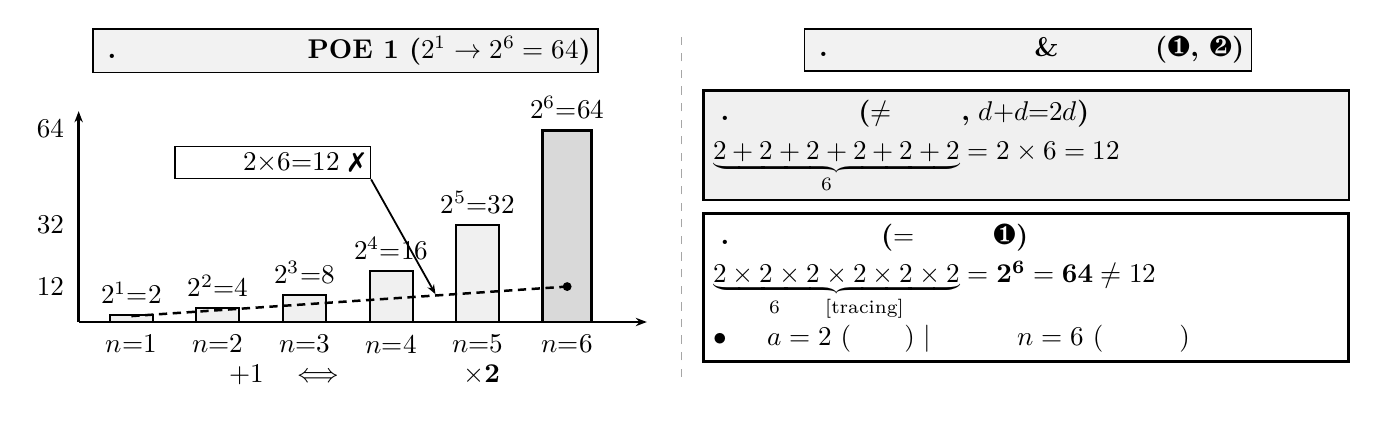
\begin{tikzpicture}[x=0.88cm, y=0.75cm, every node/.style={font=\linespread{1.0}\fontsize{9.8pt}{12.5pt}\selectfont, text=black}]
  \draw[line width=0.6pt, dashed, gray!70] (9.55, 0.05) -- (9.55, 5.95);
  \node[anchor=north, fill=headgray, draw=black, line width=0.5pt, inner sep=2.6pt] at (4.70, 5.95) {\textbf{ក\en{.} ពិសោធន៍បត់ក្រដាសទ្វេដង \en{POE 1} ($2^1 \to 2^6 = 64$)}};
  \node[anchor=north, fill=headgray, draw=black, line width=0.5pt, inner sep=2.6pt] at (14.55, 5.95) {\textbf{ខ\en{.} កម្ទេចអន្ទាក់គុណលីនេអ៊ែរ \en{\&} អន្ទាក់បូក (\cnum{1}, \cnum{2})}};

  % Left: Stepped bar chart of 2^1..2^6 vs dashed linear line 2n
  \draw[black, line width=0.85pt, -{Stealth[length=4pt]}] (0.85, 0.98) -- (9.05, 0.98);
  \draw[black, line width=0.85pt, -{Stealth[length=4pt]}] (0.85, 0.98) -- (0.85, 4.55);
  \node[anchor=east] at (0.78, 4.25) {\en{64}};
  \node[anchor=east] at (0.78, 2.62) {\en{32}};
  \node[anchor=east] at (0.78, 1.58) {\en{12}};

  % Bars for n=1..6 (clear >= 3.5mm below header box)
  \fill[panelgray, draw=black, line width=0.75pt] (1.30, 0.98) rectangle (1.92, 1.10);
  \node[anchor=south] at (1.61, 1.12) {\en{$2^1{=}2$}};
  \node[anchor=north] at (1.61, 0.93) {\en{$n{=}1$}};

  \fill[panelgray, draw=black, line width=0.75pt] (2.55, 0.98) rectangle (3.17, 1.22);
  \node[anchor=south] at (2.86, 1.24) {\en{$2^2{=}4$}};
  \node[anchor=north] at (2.86, 0.93) {\en{$n{=}2$}};

  \fill[panelgray, draw=black, line width=0.75pt] (3.80, 0.98) rectangle (4.42, 1.44);
  \node[anchor=south] at (4.11, 1.46) {\en{$2^3{=}8$}};
  \node[anchor=north] at (4.11, 0.93) {\en{$n{=}3$}};

  \fill[panelgray, draw=black, line width=0.75pt] (5.05, 0.98) rectangle (5.67, 1.84);
  \node[anchor=south] at (5.36, 1.86) {\en{$2^4{=}16$}};
  \node[anchor=north] at (5.36, 0.93) {\en{$n{=}4$}};

  \fill[panelgray, draw=black, line width=0.75pt] (6.30, 0.98) rectangle (6.92, 2.62);
  \node[anchor=south] at (6.61, 2.64) {\en{$2^5{=}32$}};
  \node[anchor=north] at (6.61, 0.93) {\en{$n{=}5$}};

  \fill[stepgray, draw=black, line width=1.05pt] (7.55, 0.98) rectangle (8.25, 4.22);
  \node[anchor=south] at (7.90, 4.25) {\textbf{\en{$2^6{=}64$}}};
  \node[anchor=north] at (7.90, 0.93) {\textbf{\en{$n{=}6$}}};

  % Dashed linear trap line 2*n with non-overlapping callout box in open upper-left space
  \draw[black, densely dashed, line width=0.9pt] (1.61, 1.08) -- (7.90, 1.58);
  \fill[black] (7.90, 1.58) circle (1.6pt);
  \node[draw=black, line width=0.55pt, fill=white, inner sep=2.2pt] (TRAP) at (3.65, 3.68) {អន្ទាក់ $2{\times}6{=}12$ \ding{55}};
  \draw[black, line width=0.65pt, -{Stealth[length=3.5pt]}] (TRAP.south east) -- (6.00, 1.45);
  \node[anchor=north, align=center] at (4.75, 0.42) {បត់ $+1$ ដង $\Longleftrightarrow$ ស្រទាប់គុណទ្វេ $\mathbf{\times 2}$};

  % Right self-sizing boxes (zero border collision possible)
  \node[anchor=north west, draw=black, line width=0.85pt, fill=panelgray, inner sep=3.5pt, align=left, text width=7.95cm] (R1T) at (9.85, 4.92) {%
    \textbf{១\en{.} ផលបូកតួដូចគ្នា ($\neq$ ស្វ័យគុណ, $d{+}d{=}2d$)៖}\\[1.5pt]
    $\underbrace{2 + 2 + 2 + 2 + 2 + 2}_{6\text{ តួ}} = 2 \times 6 = 12$};

  \node[anchor=north west, draw=black, line width=1.05pt, fill=white, inner sep=3.5pt, align=left, text width=7.95cm, below=4pt of R1T] (R1B) {%
    \textbf{២\en{.} ផលគុណកត្តាដូចគ្នា ($=$ ស្វ័យគុណ \cnum{1})៖}\\[1.5pt]
    $\underbrace{2 \times 2 \times 2 \times 2 \times 2 \times 2}_{6\text{ កត្តា \en{[tracing]}}} = \mathbf{2^6 = 64} \neq 12$\\[1.5pt]
    $\bullet$ គោល $a=2$ (អ្នកគុណ) $\vert$ និទស្សន្ត $n=6$ (ចំនួនកត្តា)};
\end{tikzpicture}\par
\vspace{1.5pt}
{\linespread{1.02}\fontsize{10.5pt}{13.8pt}\selectfont\textbf{រូបទី ១៖} កំណើនស្វ័យគុណតាមការបត់ក្រដាសទ្វេដង ($2^6=64$) ទល់នឹងអន្ទាក់លីនេអ៊ែរ ($2\times 6=12$) និងអន្ទាក់បូកតួដូចគ្នា \en{(De Bock et al., 2003; Siller et al., 2023; Moru \& Mathunya, 2022)}។\par}
\end{tcolorbox}

\textbf{គន្លឹះដឹកនាំលើរូបទី ១ (ជំហាន \en{E1--E2})៖} គ្រូគូសបន្ទាត់ដាច់ៗនៃអន្ទាក់លីនេអ៊ែរ $2\times n$ ធៀបនឹងសសរស្វ័យគុណ $2^n$ លើក្ដារខៀនផ្នែកឆ្វេង រួចឱ្យសិស្សអូសម្រាមដៃ \en{[tracing]} រាប់កត្តាគុណពីឆ្វេងទៅស្ដាំដើម្បីទប់ស្កាត់កំហុស $d+d=d^2$ និង $2^5=10$។

% --- រូបទី ២ ---
\Needspace{1.8cm}
\begin{tcolorbox}[enhanced, sharp corners, colback=white, colframe=black, boxrule=0.8pt, top=3pt, bottom=3pt, left=4pt, right=4pt, before skip=2pt, after skip=3pt]
\centering
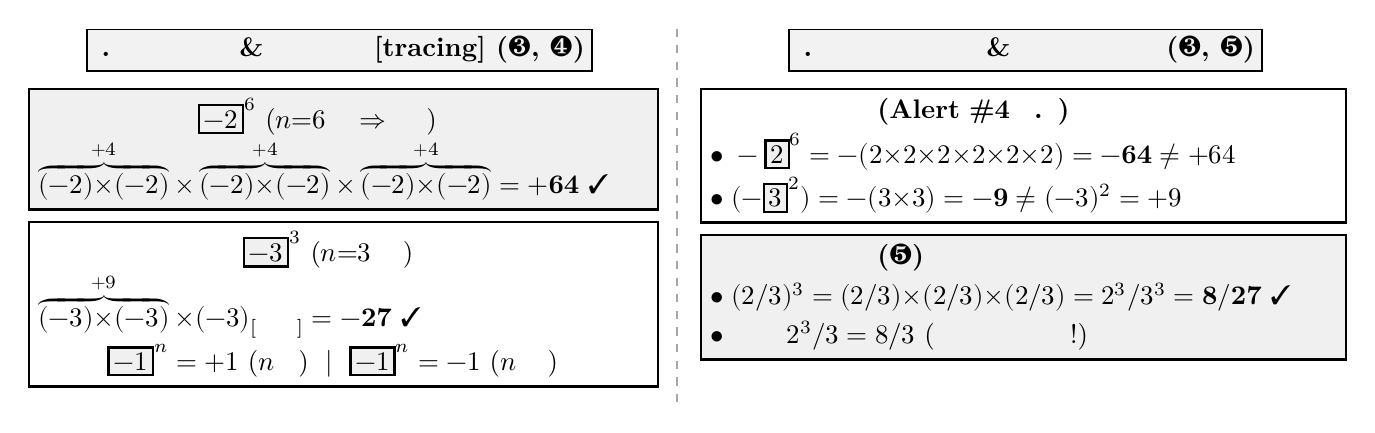
\begin{tikzpicture}[x=0.88cm, y=0.75cm, every node/.style={font=\linespread{1.0}\fontsize{9.7pt}{12.4pt}\selectfont, text=black}]
  \node[anchor=north, fill=headgray, draw=black, line width=0.5pt, inner sep=2.6pt] (H2L) at (4.65, 6.20) {\textbf{ក\en{.} ប្រអប់ចាក់សោដក \en{\&} ធ្នូផ្គូផ្គង \en{[tracing]} (\cnum{3}, \cnum{4})}};
  \node[anchor=north, fill=headgray, draw=black, line width=0.5pt, inner sep=2.6pt] (H2R) at (14.55, 6.20) {\textbf{ខ\en{.} អន្ទាក់គ្មានវង់ក្រចក \en{\&} ប្រអប់ចាក់សោប្រភាគ (\cnum{3}, \cnum{5})}};

  % Left top & bottom self-sizing boxes
  \node[anchor=north west, draw=black, line width=0.95pt, fill=panelgray, inner sep=3.4pt, align=left, text width=7.75cm] (L2T) at (0.15, 5.20) {%
    \textbf{មានវង់ក្រចកចាក់សោដក៖} $\lockbox{-2}^6$ ($n{=}6$ គូ $\Rightarrow$ ៣ គូ)\\[2pt]
    $\overbrace{(-2){\times}(-2)}^{+4}\times\overbrace{(-2){\times}(-2)}^{+4}\times\overbrace{(-2){\times}(-2)}^{+4} = \mathbf{+64}$ \ding{51}};

  \node[anchor=north west, draw=black, line width=0.85pt, fill=white, inner sep=3.4pt, align=left, text width=7.75cm, below=3.5pt of L2T] (L2B) {%
    \textbf{និទស្សន្តសេសក្នុងវង់ក្រចក៖} $\lockbox{-3}^3$ ($n{=}3$ សេស)\\[2pt]
    $\overbrace{(-3){\times}(-3)}^{+9}\times(-3)_{\text{[សល់ដក ១]}} = \mathbf{-27}$ \ding{51}\\[1.5pt]
    \textbf{សម្គាល់៖} $\lockbox{-1}^n = +1$ ($n$ គូ) $\;\vert\;$ $\lockbox{-1}^n = -1$ ($n$ សេស)};

  % Right top & bottom self-sizing boxes
  \node[anchor=north west, draw=black, line width=0.95pt, fill=white, inner sep=3.4pt, align=left, text width=7.95cm] (R2T) at (9.85, 5.20) {%
    \textbf{សញ្ញាដកនៅក្រៅស្វ័យគុណ (\en{Alert \#4} ទំ\en{.}២៥)៖}\\[2pt]
    $\bullet\; -\lockbox{2}^6 = -(2{\times}2{\times}2{\times}2{\times}2{\times}2) = \mathbf{-64} \neq +64$\\[1.5pt]
    $\bullet\; (-\lockbox{3}^2) = -(3{\times}3) = \mathbf{-9} \neq (-3)^2 = +9$};

  \node[anchor=north west, draw=black, line width=0.85pt, fill=panelgray, inner sep=3.4pt, align=left, text width=7.95cm, below=3.5pt of R2T] (R2B) {%
    \textbf{ប្រអប់ចាក់សោគោលប្រភាគ (\cnum{5})៖}\\[2pt]
    $\bullet\; (2/3)^3 = (2/3){\times}(2/3){\times}(2/3) = 2^3/3^3 = \mathbf{8/27}$ \ding{51}\\[1.5pt]
    $\bullet\;$ ខុសពី $2^3/3 = 8/3$ (លើកស្វ័យគុណតែភាគយក!)};

  \draw[line width=0.6pt, dashed, gray!70] (9.52, 6.20) -- (9.52, -0.15);
\end{tikzpicture}\par
\vspace{1.5pt}
{\linespread{1.02}\fontsize{10.5pt}{13.8pt}\selectfont\textbf{រូបទី ២៖} យន្តការប្រអប់ចាក់សោវង់ក្រចក និងធ្នូផ្គូផ្គងសញ្ញាដក \en{[tracing]} ញែកដាច់ $(-2)^6$ ពី $-2^6$, $(-3^2)$ និង $(2/3)^3$ ពី $2^3/3$ \en{(Ulusoy, 2019; Theba et al., 2024; Bye et al., 2024)}។\par}
\end{tcolorbox}

\textbf{គន្លឹះដឹកនាំលើរូបទី ២ (ជំហាន \en{E2 POE 2 \& E4})៖} មុនពេលសិស្សគណនាស្វ័យគុណដែលមានសញ្ញាដក ឬប្រភាគ គ្រូតម្រូវឱ្យសិស្សសួរខ្លួនឯងជាមុនថា \textit{«តើនិទស្សន្តឈរពីលើតួណាខ្លះ?»} រួចគូសប្រអប់បួនជ្រុង \lockbox{\cdots} ចាក់សោតួនោះសិន។ បើសញ្ញាដកស្ថិតនៅក្រៅប្រអប់ (ដូចជា $-2^6$ ឬ $(-3^2)$ ក្នុងលំហាត់ទំ\en{.}២៥ \en{\#3}ក) សញ្ញាដកនោះត្រូវរង់ចាំនៅខាងមុខរហូតគណនាស្វ័យគុណចប់!

% --- រូបទី ៣ ---
\Needspace{1.8cm}
\begin{tcolorbox}[enhanced, sharp corners, colback=white, colframe=black, boxrule=0.8pt, top=3pt, bottom=3pt, left=4pt, right=4pt, before skip=2pt, after skip=3pt]
\centering
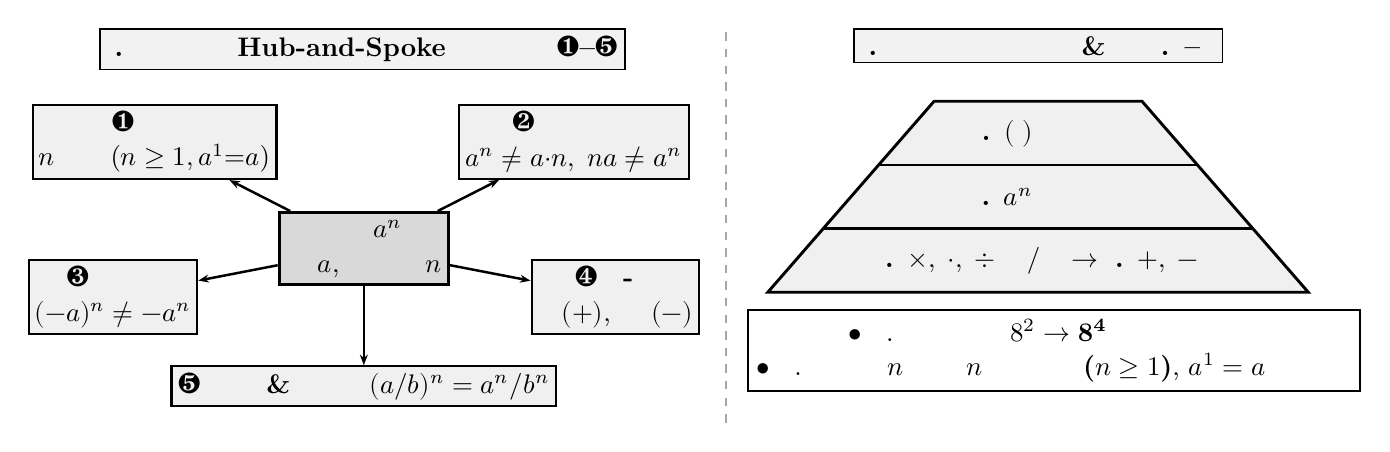
\begin{tikzpicture}[x=0.88cm, y=0.77cm, every node/.style={font=\linespread{1.0}\fontsize{9.7pt}{12.4pt}\selectfont, text=black}]
  \draw[line width=0.6pt, dashed, gray!70] (10.35, -0.05) -- (10.35, 6.45);
  \node[anchor=north, fill=headgray, draw=black, line width=0.5pt, inner sep=2.6pt] at (5.10, 6.45) {\textbf{ក\en{.} រចនាសម្ព័ន្ធ \en{Hub-and-Spoke} ធនាគារហេតុផល \cnum{1}\en{--}\cnum{5}}};
  \node[anchor=north, fill=headgray, draw=black, line width=0.5pt, inner sep=2.6pt] at (14.85, 6.45) {\textbf{ខ\en{.} ត្រីកោណអាទិភាពប្រមាណវិធី \en{\&} កំណែទំ\en{.}១៣\en{--}១៤}};

  % Left: Hub-and-Spoke Diagram around Central Hub a^n (generous clearance below header & side spokes)
  \node[draw=black, line width=1.15pt, fill=stepgray, align=center, inner sep=2.6pt] (HUB) at (5.12, 2.82) {\textbf{ស្នូល $a^n$}\\ គោល $a$, និទស្សន្ត $n$};

  \node[draw=black, line width=0.75pt, fill=panelgray, align=center, inner sep=2.3pt] (S1) at (2.10, 4.58) {\textbf{\cnum{1} និយមន័យ}\\ $n$ កត្តា ($n\ge 1, a^1{=}a$)};
  \node[draw=black, line width=0.75pt, fill=panelgray, align=center, inner sep=2.3pt] (S2) at (8.15, 4.58) {\textbf{\cnum{2} របាំងអន្ទាក់}\\ $a^n\neq a{\cdot}n,\; na\neq a^n$};
  \node[draw=black, line width=0.75pt, fill=panelgray, align=center, inner sep=2.2pt] (S3) at (1.50, 2.02) {\textbf{\cnum{3} ប្រអប់ដក}\\ $(-a)^n \neq -a^n$};
  \node[draw=black, line width=0.75pt, fill=panelgray, align=center, inner sep=2.2pt] (S4) at (8.75, 2.02) {\textbf{\cnum{4} គូ-សេស}\\ គូ $(+)$, សេស $(-)$};
  \node[draw=black, line width=0.75pt, fill=panelgray, align=center, inner sep=2.3pt] (S5) at (5.12, 0.55) {\textbf{\cnum{5} ប្រភាគ \en{\&} អាទិភាព}៖ $(a/b)^n = a^n/b^n$};

  \draw[black, line width=0.9pt, -{Stealth[length=3.8pt]}] (HUB) -- (S1);
  \draw[black, line width=0.9pt, -{Stealth[length=3.8pt]}] (HUB) -- (S2);
  \draw[black, line width=0.9pt, -{Stealth[length=3.8pt]}] (HUB) -- (S3);
  \draw[black, line width=0.9pt, -{Stealth[length=3.8pt]}] (HUB) -- (S4);
  \draw[black, line width=0.9pt, -{Stealth[length=3.8pt]}] (HUB) -- (S5);

  % Right: Trapezoid/Wide Pyramid so top tier cleanly encloses "១. ( ) វង់ក្រចក"
  \coordinate (Ptl) at (13.35, 5.25);
  \coordinate (Ptr) at (16.35, 5.25);
  \coordinate (Pbl) at (10.95, 2.10);
  \coordinate (Pbr) at (18.75, 2.10);
  \fill[panelgray] (Ptl) -- (Ptr) -- (Pbr) -- (Pbl) -- cycle;
  \draw[black, line width=1.05pt] (Ptl) -- (Ptr) -- (Pbr) -- (Pbl) -- cycle;
  \draw[black, line width=0.8pt] (12.55, 4.20) -- (17.15, 4.20);
  \draw[black, line width=0.8pt] (11.75, 3.15) -- (17.95, 3.15);
  \node[align=center] at (14.85, 4.72) {\textbf{១\en{.} $( \; )$} វង់ក្រចក};
  \node[align=center] at (14.85, 3.67) {\textbf{២\en{.} $a^n$} ស្វ័យគុណ};
  \node[align=center] at (14.85, 2.62) {\textbf{៣\en{.} $\times,\;\cdot,\;\div$} គុណ/ចែក $\to$ \textbf{៤\en{.} $+,\;-$}};

  \node[anchor=north west, draw=black, fill=white, line width=0.8pt, inner sep=3.2pt, align=left, text width=7.55cm] at (10.65, 1.82) {%
    \textbf{កែសៀវភៅគោល៖} $\bullet$ ទំ\en{.}១៣ បន្ទាត់ ១៤៖ $8^2 \to \mathbf{8^4}$\\
    $\bullet$ ទំ\en{.}១៤ និយមន័យ $n$ កត្តា៖ $n$ \textbf{គត់វិជ្ជមាន ($n\ge 1$)}, $a^1=a$};
\end{tikzpicture}\par
\vspace{1.5pt}
{\linespread{1.02}\fontsize{10.5pt}{13.8pt}\selectfont\textbf{រូបទី ៣៖} រចនាសម្ព័ន្ធពុទ្ធិ \en{Hub-and-Spoke} នៃធនាគារហេតុផល \cnum{1}\en{--}\cnum{5} ឋានានុក្រមប្រមាណវិធី និងកំណែទំព័រ ១៣\en{--}១៤ \en{(Xu et al., 2026; Ali Rahman et al., 2017; Sureda \& Otero, 2019)}។\par}
\end{tcolorbox}

\textbf{គន្លឹះដឹកនាំលើរូបទី ៣ (ជំហាន \en{E3})៖} ការបិទផ្ទាំង \en{Hub-and-Spoke} នៅកណ្ដាលក្ដារខៀនជួយឱ្យសិស្សចងភ្ជាប់ក្បួនទាំង ៥ ទៅនឹងអត្ថន័យស្នូលតែមួយនៃ $a^n$ ជំនួសការទន្ទេញច្បាប់ដាច់ៗពីគ្នា។ គ្រូគួរឱ្យសិស្សចង្អុលលេខកូដ \cnum{1}\en{--}\cnum{5} រាល់ពេលឡើងបកស្រាយចម្លើយនៅជំហាន \en{E4} និង \en{E5}។

% --- រូបទី ៤ ---
\Needspace{1.8cm}
\begin{tcolorbox}[enhanced, sharp corners, colback=white, colframe=black, boxrule=0.8pt, top=3pt, bottom=3pt, left=4pt, right=4pt, before skip=2pt, after skip=3pt]
\centering
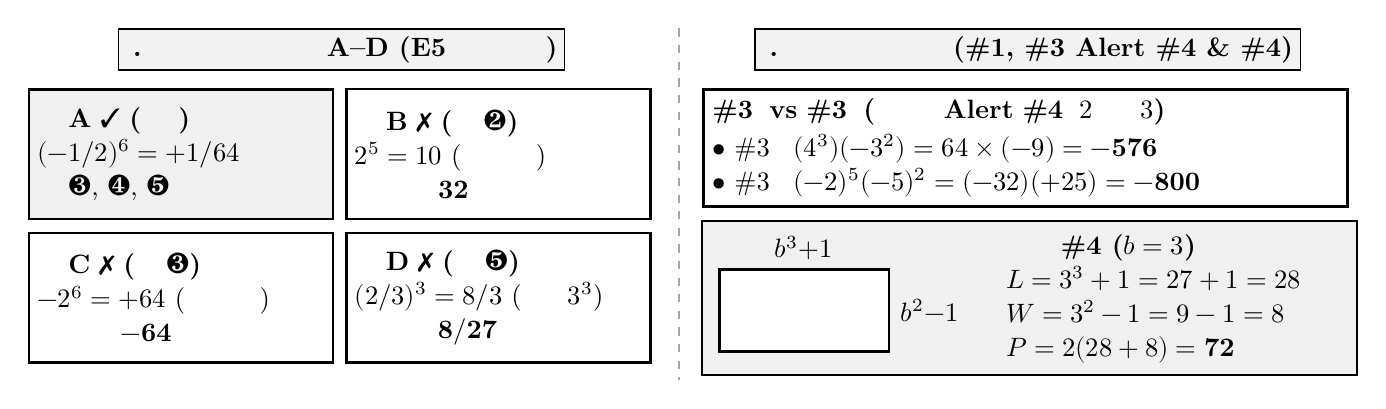
\begin{tikzpicture}[x=0.88cm, y=0.77cm, every node/.style={font=\linespread{1.0}\fontsize{9.6pt}{12.3pt}\selectfont, text=black}]
  \node[anchor=north, fill=headgray, draw=black, line width=0.5pt, inner sep=2.6pt] at (4.65, 6.00) {\textbf{ក\en{.} កាតវិនិច្ឆ័យ ៤ ទម្រង់ \en{A--D} (\en{E5} វាយតម្លៃរហ័ស)}};
  \node[anchor=north, fill=headgray, draw=black, line width=0.5pt, inner sep=2.6pt] at (14.55, 6.00) {\textbf{ខ\en{.} កិច្ចការផ្ទះទំព័រ ២៥ (\en{\#1, \#3 Alert \#4 \& \#4})}};

  % Left 2x2 self-sizing Diagnostic Cards A-D
  \node[anchor=north west, draw=black, line width=0.95pt, fill=panelgray, inner sep=3.0pt, align=left, text width=3.65cm, minimum height=1.65cm] (CA) at (0.12, 5.02) {%
    \textbf{កាត \en{A} \ding{51} (ត្រូវ)}\\ $(-1/2)^6 = +1/64$\\ តាម \cnum{3}, \cnum{4}, \cnum{5}};

  \node[anchor=north west, draw=black, line width=0.85pt, fill=white, inner sep=3.0pt, align=left, text width=3.65cm, minimum height=1.65cm, right=4pt of CA] (CB) {%
    \textbf{កាត \en{B} \ding{55} (ខុស \cnum{2})}\\ $2^5 = 10$ (អន្ទាក់គុណ)\\ ចម្លើយពិត៖ $\mathbf{32}$};

  \node[anchor=north west, draw=black, line width=0.85pt, fill=white, inner sep=3.0pt, align=left, text width=3.65cm, minimum height=1.65cm, below=4pt of CA] (CC) {%
    \textbf{កាត \en{C} \ding{55} (ខុស \cnum{3})}\\ $-2^6 = +64$ (គ្មានក្រចក)\\ ចម្លើយពិត៖ $\mathbf{-64}$};

  \node[anchor=north west, draw=black, line width=0.85pt, fill=white, inner sep=3.0pt, align=left, text width=3.65cm, minimum height=1.65cm, right=4pt of CC] (CD) {%
    \textbf{កាត \en{D} \ding{55} (ខុស \cnum{5})}\\ $(2/3)^3 = 8/3$ (ភ្លេច $3^3$)\\ ចម្លើយពិត៖ $\mathbf{8/27}$};

  % Right top self-sizing box: Alert #4 on #3a vs #3b
  \node[anchor=north west, draw=black, line width=0.95pt, fill=white, inner sep=3.3pt, align=left, text width=7.95cm] (R4T) at (9.85, 5.02) {%
    \textbf{\en{\#3}ក \en{vs \#3}ខ (ប្រយ័ត្ន \en{Alert \#4}៖ $2$ លើតែ $3$)៖}\\[1.5pt]
    $\bullet$ \en{\#3}ក៖ $(4^3)(-3^2) = 64 \times (-9) = \mathbf{-576}$\\
    $\bullet$ \en{\#3}ខ៖ $(-2)^5(-5)^2 = (-32)(+25) = \mathbf{-800}$};

  % Right bottom box: Exercise #4 Rectangle Perimeter Diagram (generous inner clearance)
  \draw[black, line width=0.85pt, fill=panelgray] (9.85, 0.28) rectangle (19.30, 2.82);
  \draw[black, line width=1.05pt, fill=white] (10.10, 0.68) rectangle (12.55, 2.02);
  \node[anchor=south] at (11.32, 2.02) {\en{$b^3{+}1$}};
  \node[anchor=west] at (12.58, 1.35) {\en{$b^2{-}1$}};
  \node[anchor=west, align=left] at (14.10, 1.54) {\textbf{លំហាត់ \en{\#4} ($b=3$)៖}\\ $L = 3^3+1 = 27+1 = 28$\\ $W = 3^2-1 = 9-1 = 8$\\ $P = 2(28+8) = \mathbf{72}$};

  \draw[line width=0.6pt, dashed, gray!70] (9.52, 6.00) -- (9.52, 0.20);
\end{tikzpicture}\par
\vspace{1.5pt}
{\linespread{1.02}\fontsize{10.5pt}{13.8pt}\selectfont\textbf{រូបទី ៤៖} កាតវិនិច្ឆ័យកំហុស \en{A--D} សម្រាប់ជំហាន \en{E5} និងគំនូសណែនាំកិច្ចការផ្ទះទំព័រ ២៥ (\en{\#3} និង \en{\#4} ចតុកោណកែង) \en{(Booth et al., 2013; Bye et al., 2024; Tabak, 2019)}។\par}
\end{tcolorbox}

\textbf{គន្លឹះដឹកនាំលើរូបទី ៤ (ជំហាន \en{E5 \&} ជំហានទី ៥)៖} នៅនាទីទី ៤៤\en{.}៥ គ្រូលើកកាត \en{A--D} ឱ្យសិស្សធ្វើសញ្ញាដៃរួមគ្នាដើម្បីស្ទង់មើលថាតើនៅសល់សិស្សប៉ុន្មានភាគរយដែលច្រឡំ $-2^6$ ឬភ្លេចលើកភាគបែងប្រភាគ មុននឹងចែកសំបុត្រចេញ និងផ្ដាំកិច្ចការផ្ទះទំព័រ ២៥។

% ============================================================================
% ផ្នែកទី ៦៖ គម្រោងសម្ភារៈបោះពុម្ព ចម្លើយគំរូ និងផែនការបម្រុងពេលវេលា
% ============================================================================
\secbanner{ផ្នែកទី ៦៖ គម្រោងសម្ភារៈបោះពុម្ព ចម្លើយគំរូ និងការត្រៀមមុនបង្រៀន}{Section 6: Planned Printable Suite Blueprint (Pages 1--6), Complete Master Answer Keys \& Pre-Flight Plan}

\subsec{៦\enbf{.}១ គម្រោងសម្ភារៈបោះពុម្ព ស\enbf{-}ខ្មៅ ទាំង ៦ ទំព័រ \enbf{(Blueprint for Next Phase)}}

នៅពេលរៀបចំកិច្ចតែងការបង្រៀន (\en{LS\_Plan\_EXP1}) និងសម្ភារៈបោះពុម្ព (\en{Printable\_Materials\_EXP1}) ក្នុងជំហានបន្ទាប់ កញ្ចប់សន្លឹកកិច្ចការ ស-ខ្មៅ នឹងរៀបចំជា ៦ ទំព័រ \en{A4} ដាច់ៗពីគ្នា៖
\begin{enumerate}[leftmargin=0.65cm, itemsep=1.5pt]
  \item \textbf{ទំព័រ ១ (\en{E2 Lab — Actual Size 100\%} + បន្ទះក្រិត \en{5.00 cm})៖} ពុម្ពបន្ទះក្រដាសបត់ខ្នាត \en{1:1} ($16.00\unit{cm}\times 3.00\unit{cm}$ មានខ្សែបត់ \en{F1--F4}) + តារាងកត់ត្រា \en{POE 1} ($n=1\dots 6$) + សន្លឹកពិសោធន៍ប្រអប់ចាក់សោ \en{POE 2} ($\lockbox{-2}^6$ \en{vs} $-2^6$, $(-3)^3$, $(\frac{2}{3})^3$ \en{vs} $\frac{2^3}{3}$)។
  \item \textbf{ទំព័រ ២ (\en{E4} កាតស៊ើបអង្កេត \en{2-up})៖} លំហាត់គំរូទី ១ ($4^6, a^{2010}$) និងគំរូទី ២ ($2^5, (\frac{2}{3})^3, (-3)^3, (-2)^6$ ធៀបនឹង $-2^6$ \en{\&} $(-3^2)$) + សំណួរ \en{EIA 30s}។
  \item \textbf{ទំព័រ ៣ (\en{E5} សន្លឹក \en{Relay} ៣ តួនាទី \en{2-up})៖} ប្រតិបត្តិ ១ ($x^6, y^{2013}$) និងប្រតិបត្តិ ២ ($3^4, (-\frac{1}{2})^6, (-2)^7$) ភ្ជាប់ \en{Pause-Ask}, \en{Pause-Review!} និងការឆ្លើយបិទបេសកកម្ម \en{E1}។
  \item \textbf{ទំព័រ ៤ (\en{Anchor Poster 1-up})៖} ផ្ទាំងធនាគារហេតុផល \cnum{1}\en{--}\cnum{5}, ត្រីកោណអាទិភាព និងកំណែទំ\en{.}១៣\en{--}១៤ សម្រាប់បិទលើក្ដារខៀន។
  \item \textbf{ទំព័រ ៥ (\en{E5} កាត \en{A--D} + សំបុត្រចេញ \en{2-up})៖} កាតវិនិច្ឆ័យ \en{A--D} និងសំបុត្រចេញ ៦០\en{--}៩០ វិនាទី ចំនួន ៣ សំណួរ។
  \item \textbf{ទំព័រ ៦ (ប័ណ្ណកិច្ចការផ្ទះ \en{4-up})៖} ទំ\en{.}២៥ \en{\#1}(ក\en{--}ឃ), \en{\#3}(ក\en{,} ខ\en{,} ឃ) ភ្ជាប់ប្រអប់ព្រមាន \en{Alert \#4} និង \en{\#4} ($b=3$)។
\end{enumerate}

\Needspace{2.1cm}
\subsec{៦\enbf{.}២ ចម្លើយគំរូពេញលេញសម្រាប់គ្រប់លំហាត់សៀវភៅគោល និងសន្លឹកកិច្ចការ \enbf{(Master Answer Key)}}

\begingroup
\linespread{1.02}\fontsize{10.1pt}{14.4pt}\selectfont
\renewcommand{\arraystretch}{1.06}
\begin{longtable}{|L{3.10cm}|L{14.30cm}|}
\hline
\rowcolor{headgray}
\multicolumn{1}{|C{3.10cm}|}{\tblhead{ផ្នែក \enbf{/} លំហាត់}} &
\multicolumn{1}{C{14.30cm}|}{\tblhead{ចម្លើយគំរូផ្លូវការ ជំហានគណនា និងលេខកូដសំអាង \enbf{(Master Key)}}} \\
\hline
\endfirsthead
\hline
\rowcolor{headgray}
\multicolumn{1}{|C{3.10cm}|}{\tblhead{ផ្នែក \enbf{/} លំហាត់}} &
\multicolumn{1}{C{14.30cm}|}{\tblhead{ចម្លើយគំរូផ្លូវការ ជំហានគណនា និងលេខកូដសំអាង \enbf{(Master Key)}}} \\
\hline
\endhead
\hline
\endfoot
\hline
\endlastfoot
\textbf{ពិសោធន៍ \en{E2}} \newline (\en{POE 1 \& POE 2}) &
\textbf{\en{POE 1} (បត់ក្រដាស ១\en{--}៦ ដង)៖} $n=1\to 2^1=2$; $n=2\to 2^2=4$; $n=3\to 2^3=8$; $n=4\to 2^4=16$; $n=5\to 2^5=32$; $n=6\to \mathbf{2^6=64\text{ ស្រទាប់}}$ ($\neq 2\times 6=12$, តាម \cnum{1}, \cnum{2})។ \\[2pt]
& \textbf{\en{POE 2} (ប្រអប់ចាក់សោ)៖} $\lockbox{-2}^6 = +64$ (៣ គូបូក \cnum{3}, \cnum{4}) $\neq -2^6 = -(2^6) = -64$; $\lockbox{-3}^3 = -27$ (១ គូបូក សល់ដក ១); $\lockbox{\frac{2}{3}}^3 = \frac{8}{27} \neq \frac{2^3}{3} = \frac{8}{3}$ (\cnum{5})។ \\
\hline
\textbf{លំហាត់គំរូ ១\en{--}២} \newline (ទំ\en{.}១៤ \en{\& E4}) &
\textbf{គំរូទី ១៖} \textbf{ក\en{.}} $4\times 4\times 4\times 4\times 4\times 4 = \mathbf{4^6}$ (គោល $4$, និទស្សន្ត $6$, \cnum{1}); \textbf{ខ\en{.}} $\underbrace{a\times\dots\times a}_{2010\text{ កត្តា}} = \mathbf{a^{2010}}$ (គោល $a$, និទស្សន្ត $2010$, \cnum{1}, \cnum{2})។ \\[2pt]
& \textbf{គំរូទី ២៖} \textbf{ក\en{.}} $2^5 = \mathbf{32}$; \textbf{ខ\en{.}} $(\frac{2}{3})^3 = \mathbf{\frac{8}{27}}$ (\cnum{5}); \textbf{គ\en{.}} $(-3)^3 = \mathbf{-27}$ (\cnum{3}, \cnum{4}); \textbf{ឃ\en{.}} $(-2)^6 = \mathbf{64}$ (\cnum{3}, \cnum{4}) [ធៀបនឹង $-2^6 = \mathbf{-64}$ និង $(-3^2) = \mathbf{-9}$]។ \\
\hline
\textbf{ប្រតិបត្តិ ១\en{--}២} \newline (ទំ\en{.}១៤ \en{\& E5}) &
\textbf{ប្រតិបត្តិ ១៖} \textbf{ក\en{.}} $x\cdot x\cdot x\cdot x\cdot x\cdot x = \mathbf{x^6}$ (គោល $x$, និទស្សន្ត $6$); \textbf{ខ\en{.}} $\underbrace{y\cdot y\cdots y}_{2013\text{ កត្តា}} = \mathbf{y^{2013}}$ (គោល $y$, និទស្សន្ត $2013$, \cnum{1})។ \\[2pt]
& \textbf{ប្រតិបត្តិ ២៖} \textbf{ក\en{.}} $3^4 = 3\times 3\times 3\times 3 = \mathbf{81}$ (\cnum{1}); \textbf{ខ\en{.}} $(-\frac{1}{2})^6 = +\frac{1^6}{2^6} = \mathbf{\frac{1}{64}}$ (\cnum{3}, \cnum{4}, \cnum{5}); \textbf{គ\en{.}} $(-2)^7 = -(2^7) = \mathbf{-128}$ (\cnum{3}, \cnum{4})។ \\
\hline
\textbf{សំបុត្រចេញ \en{E5}} \newline (៦០\en{--}៩០ វិនាទី) &
\textbf{សំណួរ ១៖} គណនា $(-3)^4 = \mathbf{+81}$ និង $-3^4 = -(3^4) = \mathbf{-81}$ (\cnum{3}, \cnum{4})។ \textbf{សំណួរ ២៖} គណនា $(-\frac{2}{5})^3 = \mathbf{-\frac{8}{125}}$ (\cnum{4}, \cnum{5})។ \textbf{សំណួរ ៣៖} តើ $2^4 + 1 = 9$ ត្រូវ ឬខុស? \textbf{ខុស} (គណនា $2\times 4$ ជំនួស $2^4=16$; ចម្លើយពិត $16+1 = \mathbf{17}$ តាម \cnum{2}, \cnum{5})។ \\
\hline
\textbf{កិច្ចការផ្ទះទំ\en{.}២៥} \newline \en{\#1, \#3 \& \#4} &
\textbf{លំហាត់ទី ១ (ទម្រង់ស្វ័យគុណ)៖} \textbf{ក\en{.}} $7\times 7\times 7\times 7\times 7 = \mathbf{7^5}$; \textbf{ខ\en{.}} $\frac{1}{2}\times\frac{1}{2}\times\frac{1}{2}\times\frac{1}{2} = \mathbf{(\frac{1}{2})^4}$; \textbf{គ\en{.}} $(-0.7)\times(-0.7)\times(-0.7)\times(-0.7) = \mathbf{(-0.7)^4}$; \textbf{ឃ\en{.}} $(-\frac{3}{7})$ គុណ $5$ កត្តា $= \mathbf{(-\frac{3}{7})^5}$ (\cnum{1}, \cnum{3}, \cnum{5})។ \\[2pt]
& \textbf{លំហាត់ទី ៣ (គណនា)៖} \textbf{ក\en{.}} $(4^3)(-3^2) = 64\times[-(3^2)] = 64\times(-9) = \mathbf{-576}$ (\cnum{3}, \cnum{5}); \textbf{ខ\en{.}} $(-2)^5(-5)^2 = (-32)\times(+25) = \mathbf{-800}$ (\cnum{4}); \textbf{ឃ\en{.}} $(-4)^2(-\frac{1}{2})^3 = 16\times(-\frac{1}{8}) = \mathbf{-2}$ (\cnum{4}, \cnum{5})។ \textit{(បន្ថែមខ្ទង់ គ៖ $(-2^3)(3^2)(-5^2) = (-8)(9)(-25) = \mathbf{+1800}$)}។ \\[2pt]
& \textbf{លំហាត់ទី ៤ (បរិមាត្រចតុកោណកែងចំពោះ $b=3$)៖} បណ្ដោយ $L = b^3 + 1 = 3^3 + 1 = 27 + 1 = \mathbf{28}$; ទទឹង $W = b^2 - 1 = 3^2 - 1 = 9 - 1 = \mathbf{8}$; បរិមាត្រ $P = 2(L + W) = 2(28 + 8) = 2\times 36 = \mathbf{72}$ (\cnum{1}, \cnum{5})។ \\
\hline
\end{longtable}
\endgroup

\subsec{៦\enbf{.}៣ បញ្ជីផ្ទៀងផ្ទាត់មុនចូលបង្រៀន \enbf{(Pre-Flight)} និងផែនការបត់បែនពេលវេលា}

\begin{itemize}[leftmargin=0.65cm, itemsep=2pt]
  \item \textbf{ការត្រៀមមុនចូលថ្នាក់ (\en{Pre-Flight Checklist})៖} (១) បន្ទះក្រដាសស្ដើង \en{A4/A5} ចំនួន ១ សន្លឹកក្នុង ១ ក្រុម (និងបន្ទះធំ ១ សម្រាប់គ្រូបង្ហាញមុខថ្នាក់); (២) ផ្ទាំងធនាគារហេតុផល \cnum{1}\en{--}\cnum{5} (ទំព័រ ៤) បោះពុម្ពច្បាស់ ស-ខ្មៅ សម្រាប់បិទលើក្ដារខៀនកណ្ដាល; (៣) គូសខ្សែបែងចែកក្ដារខៀនជា ៣ ផ្នែកទុកជាមុន និងកត់ទុកទំព័រ ១៣ (បន្ទាត់ ១៤), ទំព័រ ១៤ (ប្រអប់និយមន័យ) និងទំព័រ ២៥ (\en{\#3}ក) ដើម្បីដឹកនាំសិស្សកែឱ្យរហ័ស។
  \item \textbf{ផែនការបម្រុងបើសល់ ឬខ្វះពេល (\en{Contingency Plan})៖} ប្រសិនបើការបត់ក្រដាសនៅ \en{E2} ចំណាយពេលលើស ១\en{--}២ នាទី គ្រូអាចឱ្យសិស្សបត់ផ្ទាល់ត្រឹមលើកទី ៤ ($16$ ស្រទាប់) រួចសង្កេតលំនាំគុណនឹង $2$ ទាញយកលើកទី ៥ ($32$) និងលើកទី ៦ ($64$) ដើម្បីរក្សាពេលវេលាពេញ ១០ នាទីសម្រាប់ \en{E5}។ ផ្ទុយទៅវិញ បើក្រុមខ្លះធ្វើប្រតិបត្តិ ២ ចប់មុនពេល ២ នាទី គ្រូអាចឱ្យក្រុមនោះសាកល្បងលំហាត់បន្ថែម \en{\#3}គ $(-2^3)(3^2)(-5^2) = +1800$ ជាបេសកកម្មកិត្តិយស។
\end{itemize}

% ============================================================================
% ឯកសារយោង (APA 7th Edition — 15 Verified Open-Access PDFs) & ហត្ថលេខា
% ============================================================================
\vspace{2pt}
\refbanner{ឯកសារយោង}

{\TimesEn\linespread{1.03}\selectfont\fontsize{10.8pt}{15.4pt}\selectfont
\setlength{\parskip}{3.2pt}
\everypar={\hangindent=0.85cm \hangafter=1}

Ali Rahman, E. S., Shahrill, M., Abbas, N. A., \& Tan, A. (2017). Developing students' mathematical skills involving order of operations. \textit{International Journal of Research in Education and Science}, \textit{3}(2), 373--382. \url{https://doi.org/10.21890/ijres.327896}

Booth, J. L., Barbieri, C., Eyer, F., \& Paré-Blagoev, E. J. (2014). Persistent and pernicious errors in algebraic problem solving. \textit{Journal of Problem Solving}, \textit{7}(1), 10--23. \url{https://doi.org/10.7771/1932-6246.1161}

Booth, J. L., Lange, K. E., Koedinger, K. R., \& Newton, K. J. (2013). Using example problems to improve student learning in algebra: Differentiating between correct and incorrect examples. \textit{Learning and Instruction}, \textit{25}, 24--34. \url{https://files.eric.ed.gov/fulltext/ED543090.pdf}

Bye, J. K., Chan, J. Y.-C., Closser, A. H., Lee, J.-E., Shaw, S. T., \& Ottmar, E. R. (2024). Perceiving precedence: How structure and visual cues shape algebraic syntax. \textit{Journal of Numerical Cognition}, \textit{10}, Article e14103. \url{https://doi.org/10.5964/jnc.14103}

Castillo-Garsow, C. (2013). The role of multiple modeling perspectives in students' learning of exponential growth. \textit{Mathematical Biosciences and Engineering}, \textit{10}(5--6), 1437--1453. \url{https://doi.org/10.3934/mbe.2013.10.1437}

De Bock, D., Verschaffel, L., Janssens, D., Van Dooren, W., \& Claes, K. (2003). Do realistic contexts and graphical representations always have a beneficial impact on students' performance? Negative evidence from a study on modelling non-linear geometry problems. \textit{Learning and Instruction}, \textit{13}(4), 441--463. \url{https://doi.org/10.1016/S0959-4752(02)00040-3}

Lee, H.-J., \& Boyadzhiev, I. (2020). Underprepared college students' understanding of rational numbers: Misconceptions on fraction operations and grouping symbols. \textit{International Electronic Journal of Mathematics Education}, \textit{15}(3), Article em0583. \url{https://doi.org/10.29333/iejme/7835}

Moru, E. K., \& Mathunya, M. (2022). Error analysis in learning of grade 8 algebra. \textit{Journal of Research and Advances in Mathematics Education}, \textit{7}(3), 130--144. \url{https://doi.org/10.23917/jramathedu.v7i3.16784}

Siller, H.-S., Elschenbroich, H.-J., \& Greefrath, G. (2023). Mathematical modelling of exponential growth as a rich learning environment for mathematics classrooms. \textit{ZDM -- Mathematics Education}, \textit{55}(1), 17--33. \url{https://doi.org/10.1007/s11858-022-01433-8}

Sureda, P., \& Otero, R. (2019). From the powers to the exponential function. \textit{International Electronic Journal of Mathematics Education}, \textit{14}(3), 611--617. \url{https://doi.org/10.29333/iejme/5774}

Tabak, S. (2019). 6th, 7th and 8th grade students' misconceptions about the order of operations. \textit{International Journal of Educational Methodology}, \textit{5}(3), 363--373. \url{https://doi.org/10.12973/ijem.5.3.363}

Theba, N. M., Pournara, C., \& Takker, S. (2024). Exploring learners' errors with brackets using structure sense in secondary school algebra. \textit{Pythagoras}, \textit{45}(1), Article a783. \url{https://doi.org/10.4102/pythagoras.v45i1.783}

Ulusoy, F. (2019). Serious obstacles in middle school students' learning of integer exponents. \textit{International Journal of Research in Education and Science}, \textit{5}(1), 52--69. \url{https://files.eric.ed.gov/fulltext/EJ1198050.pdf}

Xu, Z., Zou, Y., Jin, C., \& Li, L. (2026). Help students construct a hub-and-spoke cognitive structure: A key pathway to reduce burden and improve quality in mathematics classroom teaching. \textit{Frontiers in Psychology}, \textit{17}, Article 1974303. \url{https://doi.org/10.3389/fpsyg.2026.1974303}

Yeo, L.-M., \& Tzeng, Y.-T. (2019). Tracing effect in the worked examples-based learning: An exploration of individual differences in working memory capacity. \textit{Eurasia Journal of Mathematics, Science and Technology Education}, \textit{15}(10), Article em1760. \url{https://doi.org/10.29333/ejmste/105482}
\par}

\vspace{8pt}
\Needspace{2.2cm}
\hfill
\begin{minipage}{9.8cm}
  {\centering
    ថ្ងៃចន្ទ ៧កើត ខែកត្តិក ឆ្នាំមមី អដ្ឋស័ក ពុទ្ធសករាជ ២៥៧០\\[2pt]
    កំពង់ស្វាយ\en{,} ថ្ងៃទី១៦ ខែវិច្ឆិកា ឆ្នាំ២០២៦\\[3pt]
    {\muol គ្រូបង្រៀន}\par}
  \vspace{32pt}
  \hfill{\muol ហុក ប៊ុនថែន}\hspace*{1.4cm}
\end{minipage}

\end{document}
